\documentclass[10pt]{elsarticle}

  \usepackage{pgfplots}
\pgfplotsset{compat=newest}
%% the following commands are needed for some matlab2tikz features
\usetikzlibrary{plotmarks}
\usetikzlibrary{arrows.meta}
\usepgfplotslibrary{patchplots}
\usepackage{grffile}
\usepackage{amsmath}
\usepackage{lineno}


%\usepackage{fullpage}
\usepackage[top=1in, bottom=1in, left=0.8in, right=1in]{geometry}
\usepackage{multicol}
\usepackage{caption}
\usepackage{subcaption}
\usepackage{hyperref}
\usepackage{xcolor}
\usepackage{graphicx,psfrag}
\usepackage[pdf]{pstricks}

\definecolor{lightblue}{rgb}{.80,.9,1}
\newcommand{\hl}[1]
    {\par\colorbox{lightblue}{\parbox{\linewidth}{#1}}}

\newcommand{\defn}{\stackrel{\textrm{\scriptsize def}}{=}}

\setlength{\columnsep}{0.1pc}

\title{Numerical Study of The Generalised Serre-Green-Naghdi Model}
%\author{Christopher Zoppou -- \texttt{christopher.zoppou@anu.edu.au}, Dimitrios Mitsotakis -- \texttt{dmitsot@gmail.com}, Stephen Roberts -- \texttt{stephen.roberts@anu.edu.au}, Jordan Pitt}

% TIME ON EVERY PAGE AS WELL AS THE FILE NAME
\usepackage{fancyhdr}
\usepackage{currfile}
\usepackage[us,12hr]{datetime} % `us' makes \today behave as usual in TeX/LaTeX
\fancypagestyle{plain}{
\fancyhf{}
\rfoot{\emph{\footnotesize \textcopyright  Serre Notes by C. Zoppou, D. Mitsatakis and S. Roberts.}
 \\ File Name: {\currfilename} \\ Date: {\ddmmyyyydate\today} at \currenttime}
\lfoot{Page \thepage}
\renewcommand{\headrulewidth}{0pt}}
\pagestyle{plain}

\definecolor{mycolor1}{rgb}{0.00000,0.44700,0.74100}%
\definecolor{mycolor2}{rgb}{0.85000,0.32500,0.09800}%
\definecolor{mycolor3}{rgb}{0.92900,0.69400,0.12500}%
\definecolor{mycolor4}{rgb}{0.49400,0.18400,0.55600}%
\definecolor{mycolor5}{rgb}{0.46600,0.67400,0.18800}% 
\definecolor{mycolor6}{rgb}{0.30100,0.74500,0.93300}%
\definecolor{mycolor7}{rgb}{0.63500,0.07800,0.18400}%

\newcommand\T{\rule{0pt}{3ex }}       % Top table strut
\newcommand\B{\rule[-4ex]{0pt}{4ex }} % Bottom table strut

\newcommand\TM{\rule{0pt}{2.8ex }}       % Top matrix strut
\newcommand\BM{\rule[-2ex]{0pt}{2ex }} % Bottom matrix strut

\newcommand{\vecn}[1]{\boldsymbol{#1}}
\DeclareRobustCommand{\solidrule}[1][0.25cm]{\rule[0.5ex]{#1}{1.5pt}}

\DeclareRobustCommand{\dashedrule}{\mbox{%
		\solidrule[2mm]\hspace{2mm}\solidrule[2mm]}}

\DeclareRobustCommand{\tikzcircle}[1]{\tikz{\filldraw[#1] (0,0) circle (0.5ex);}}	
	
	
\DeclareRobustCommand{\squaret}[1]{\tikz{\draw[#1,thick] (0,0) rectangle (0.2cm,0.2cm);}}
\DeclareRobustCommand{\circlet}[1]{\tikz{\draw[#1,thick] (0,0) circle [radius=0.1cm];}}
\DeclareRobustCommand{\trianglet}[1]{\tikz{\draw[#1,thick] (0,0) --
		(0.25cm,0) -- (0.125cm,0.25cm) -- (0,0);}}
\DeclareRobustCommand{\crosst}[1]{\tikz{\draw[#1,thick] (0cm,0cm) --
		(0.1cm,0.1cm) -- (0cm,0.2cm) -- (0.1cm,0.1cm) -- (0.2cm,0.2cm) -- (0.1cm,0.1cm)-- (0.2cm,0cm);}}
\DeclareRobustCommand{\diamondt}[1]{\tikz{\draw[#1,thick] (0,0) --(0.1cm,0.15cm) -- (0.2cm,0cm) -- (0.1cm,-0.15cm) -- (0,0)  ;}}
\DeclareRobustCommand{\squareF}[1]{\tikz{\filldraw[#1,fill opacity= 0.3] (0,0) rectangle (0.2cm,0.2cm);}}

\begin{document}

\maketitle

\vspace{-0.3in}
\noindent
\rule{\linewidth}{0.4pt}

\tableofcontents

%-------------------------------------------------
\section{Introduction}
%-------------------------------------------------
The simulation of gravity waves in fluids plays a pivotal role in the modelling of important and interesting physical phenomena such as tsunamis, storm surges and riverine flooding. Such phenomena are routinely shallow water phenomena, where the typical water depth $H$ is much smaller than the typical wave length $\lambda$, such that shallowness parameter $\sigma = H/  \lambda \ll 1$. 

A variety of equations have been developed for waves in this shallow water regime \cite{Bonneton-Lannes-2009-16601,Madsen-Schaffer-1998}. These equations are usually characterised by the powers of $\sigma$ retained in their approximation to the full Euler equations, as well as the allowable size of the non-linearity parameter $\eta = A/H$ where $A$ is the typical wave amplitude. Important members of this family of shallow water wave models are; the shallow water wave equations (SWWE) which retains only the first power of $\sigma$ \cite{Bonneton-Lannes-2009-16601} and are fully non-linear so that $\eta  = O\left(1\right)$ and the Serre-Green-Naghdi (SGN) equations which retain the third power of $\sigma$ and are also fully non-linear \cite{Bonneton-Lannes-2009-16601}. 

There are corresponding equations for any power of $\sigma$ retained, with each power of $\sigma$ allowing for more accurate modelling of waves as the shallowness restriction is relaxed and $\sigma$ increases. However, as more powers of $\sigma$ are retained higher order derivative terms appear in the equations, which can be difficult to treat analytically and numerically. Hence, the focus on lower order $\sigma$ approximations. Particular attention has been on the linear dispersion relationship of these equations, which relates the angular frequency $\omega$ to the wave number $k$ for solutions of the linearised equations. This focus is due to the utility of the linear dispersion relationship in determining the behaviour of the corresponding non-linear equations \cite{Pitt-2018-61,Dougalis-etal-2007,Clamond-et.al-2017-245}. 

Recently, \citet{Clamond-et.al-2017-245} demonstrated a family of equations that improve the dispersion relationship of the SGN equations with only a minor increase in complexity, the so called improved SGN (iSGN). The iSGN family of equations was then expanded to the generalised SGN equations (gSGN), a family of equations that includes the SWWE, the SGN equations, the iSGN family and the regularised shallow water wave equations (rSWWE) \cite{Clamond-Dutykh-2018-237}. The rSWWE are regularised SWWE in the sense that the shocks observed in solutions of the SWWE become regularised (smoothed) shocks that are no longer discontinuous \cite{Pu-2018-1361}.

This family of equations contains many members that are of current interest to the numerical wave modelling community \cite{Clamond-et.al-2017-245,Clamond-Dutykh-2018-237}. Thus a numerical method that can solve these equations allows for a single point of comparison between the numerical solutions of many different equations of interest. We propose a method to solve the gSGN that relies on generalising the methods for the SGN equations presented by \citet{Zoppou-etal-2017}.

This numerical method is then validated against analytic solutions of the SGN and the SWWE, demonstrating its convergence rate and conservation properties. Additionally, forced solutions are used to validate that all terms in the gSGN are being accurately approximated to the correct order of accuracy. Forced solutions are necessary to validate the numerical method for the more general members of this family of equations.

Finally, using the well validated numerical method a numerical investigation into the behaviour of this family of equations for a smoothed dam-break problem is performed. This problem is of particular interest firstly, because this problem requires that the numerical method is robust in the presence of steep gradients. Secondly, the solution of steep smoothed dam-break problems requires the resolution of very high wave-number waves allowing  a comprehensive observation of the differences between members of the gSGN family. Thirdly, for the rSWWE family, the transition from regularised shocks to the discontinuous shock can be observed, numerically verifying the utility of the regularisation proposed by \citet{Clamond-Dutykh-2018-237}. 


\begin{itemize}
	\item Background
	\begin{itemize}
		\item Dispersive wave equations to model phenomena
		\item New regularisation techniques to improve dispersive properties without requiring additional higher derivative terms (Denys - improved dispersion paper)
		\item Regularisation techniques to produce regularised shock waves - (other denys paper)
		\item The equations capture this new areas whilst possessing conservation law forms
		\item Such generalised equations will allow us to gain insight into heuristic processes such as switching off dispersion/ regularisation
	\end{itemize}
\item Contributions
\begin{itemize}
	\item Numerical illustrations, but no concrete methods with validation in literature
	\item Robust numerical method
	\item Numerical study of effect of beta values, in particular for various interesting classes
\end{itemize}
\end{itemize}



%-------------------------------------------------
\section{Generalised Serre-Green-Naghdi Equations}
%-------------------------------------------------
The gSGN equations derived by \citet{Clamond-Dutykh-2018-237} generalise the SGN equations that describe a depth averaged approximation to the Euler equations where $h$ is the height of the free-surface of the water, $u$ is the depth averaged velocity and $g$ is the acceleration due to gravity. The gSGN equations accomplish this by introducing two free parameters $\beta_1$ and $\beta_2$, that when fixed result in a particular member of this family of equations. The gSGN equations are particularly desirable due to their possession  of equations describing conservation of mass, momentum and energy ($\mathcal{E}$) like so:
\begin{subequations}
\begin{align}
\begin{split}
\dfrac{\partial h}{\partial t} + \dfrac{\partial (hu)}{\partial x} = 0
\label{eq:gSGNh}
\end{split}\\
\begin{split}
\dfrac{\partial (hu)}{\partial t} + \dfrac{\partial }{\partial x} \left( hu^2 + \frac{1}{2}gh^2 + \frac{1}{3} h^2 \Gamma \right)= 0
\label{eq:gSGNuh}
\end{split}\\
\begin{split}
\dfrac{\partial\left(\mathcal{E}\right)}{\partial t} +\dfrac{\partial}{\partial x}\left[hu\left(\frac{1}{2}u^2 + \dfrac{1}{4}\left(\frac{2}{3} + \beta_1\right)h^2\dfrac{\partial u}{\partial x}\dfrac{\partial u}{\partial x} + gh\left(1 + \frac{1}{4}\beta_2\dfrac{\partial h}{\partial x}\dfrac{\partial h}{\partial x} \right)   + \frac{1}{3} h\Gamma  \right) + \frac{1}{2}\beta_2 g h^3\dfrac{\partial h}{\partial x}\dfrac{\partial u}{\partial x} \right] = 0
\label{eq:gSGNE}
\end{split}
\end{align}
where
\begin{align}
\Gamma &= \frac{3}{2}\left(\frac{2}{3} + \beta_1\right)h \left[\frac{\partial u}{\partial x}\frac{\partial u}{\partial x} - \frac{\partial^2 u}{\partial x \partial t} - u\frac{\partial^2 u}{\partial x^2}\right] - \frac{3}{2} \beta_2 g\left[h \frac{\partial^2 h}{\partial x^2} + \frac{1}{2} \frac{\partial h}{\partial x}\frac{\partial h}{\partial x} \right]\\
\mathcal{E} &=\frac{1}{2}hu^2 + \dfrac{1}{4}\left(\frac{2}{3} + \beta_1\right) h^3 \dfrac{\partial u}{\partial x}\dfrac{\partial u}{\partial x} + \frac{1}{2}gh^2\left(1 + \frac{1}{2}\beta_2 \dfrac{\partial h}{\partial x} \dfrac{\partial h}{\partial x}\right) 
\end{align}
\label{eq:gSGN}
\end{subequations}

The important members (pairs of $\beta$ values) and families (groups of pairs of $\beta$ values) are summarised in Table \ref{Tab:gSGNFamilyMembers}. Equations \eqref{eq:gSGN} hold for all $\beta$ values provided the solutions are sufficiently smooth. However, for particular $\beta$ values, for example those corresponding to the SWWE, it is possible to obtain non-smooth solutions for any pair of these equations that no longer satisfy all three equations simultaneously \cite{Pu-2018-1361}. This particular issue with the SWWE, is one of reasons for the interest in regularisation techniques. 
\begin{table}
	\centering
	\begin{tabular}{l | c | c}
		Resulting Equations &$\beta_1$ & $\beta_2$  \\
		\hline 
		\T SGN Equations & $0$ & $0$ \\
		\T SWWE & $-\dfrac{2}{3}$ & $0$ \\
		\T rSWWE Family & free variable & $\beta_1 + \dfrac{2}{3}$  \\
		\T iSGN Family & free variable & $\beta_1$ \\
		\T SGN to SWWE Family & $ -\frac{2}{3}\le\beta_1 \le 0$ & $0$
	\end{tabular}
	\caption{Important members and families of equations of the gSGN in terms of the associated $\beta$ values. Here free variable, indicates that any chosen value of $\beta_1$ is a member of the family, provided that $\beta_2$ is defined in terms of $\beta_1$ in the corresponding way.}
	\label{Tab:gSGNFamilyMembers}
\end{table}

Since \eqref{eq:gSGN} are in conservation law form, when all solutions are sufficiently smooth and thus all equations hold simultaneously, the total amounts of all quantities remain constant in time. This can be seen by integrating \eqref{eq:gSGN} over the domain, and observing that the temporal derivative of the spatial integrals of mass ($h$), momentum ($uh$) and energy ($\mathcal{E}$) is zero when there is no flux across the domain boundaries. The conservation properties of numerical solutions will be used to validate the numerical method and its solutions. 

\subsection{Dispersion Relation of Linearised gSGN}
The linear dispersion properties of water wave equations has been of particular interest \cite{Filippini-etal-2016-381,Clamond-et.al-2017-245,DoCarmo-2019-125}, as the scope of modelling expands into higher order $\sigma$ equations. The gSGN equations \eqref{eq:gSGN} are linearised for small waves on a mean flow depth $h_0$ and mean flow velocity $u_0$, by seeking travelling wave solutions of the form $\exp\left(i (k x - \omega t)\right)$ as was done by \citet{Zoppou-etal-2017} to obtain
\begin{equation}
\omega^\pm = u_0 k \pm k \sqrt{gh_0} \sqrt{\dfrac{\beta_2 h_0^2 k^2 + 2}{\left(\frac{2}{3} + \beta_1\right) h_0^2 k^2 + 2} }.
\label{eq:DispRelgSGN}
\end{equation}
This dispersion relation provides the angular frequency $\omega$ of travelling wave solutions of the linearised gSGN equations for waves with wavenumber $k$. The dispersion relation has a positive and negative branch, denoted by the superscript on $\omega$. This dispersion relation \eqref{eq:DispRelgSGN} is equivalent to the dispersion relation derived by \citet{Clamond-Dutykh-2018-237} for the gSGN when $u_0 = 0$. 

From the dispersion relation \eqref{eq:DispRelgSGN}, the phase speed $v_p$ and the group speed $v_g$ can be derived as follows
\begin{subequations}
\begin{align}
v^\pm_p &= \frac{\omega^\pm}{k} = u_0 \pm  \sqrt{gh_0} \sqrt{\dfrac{\beta_2 h_0^2 k^2 + 2}{\left( \left(\frac{2}{3} + \beta_1\right) h_0^2 k^2 + 2\right)} },\\
v^\pm_g &= \frac{\partial \omega^\pm }{\partial k}= u_0  \pm  \sqrt{gh_0} \sqrt{\dfrac{\beta_2 h_0^2 k^2 + 2}{\left( \left(\frac{2}{3} + \beta_1\right) h_0^2 k^2 + 2\right)} } \left[1 +  \dfrac{\beta_2 - \left(\beta_1 + \frac{2}{3}\right)}{\left(\frac{1}{2}\beta_2 h_0^2 k^2 +1\right)\left( \left(\frac{1}{3} + \beta_1\right) h_0^2 k^2 + 1\right)}\right].
\end{align}
\label{eq:wavespeeds}
\end{subequations}
For the appropriate choices of $\beta$ values the dispersion relationship and thus the phase and group speeds of the SGN \cite{Zoppou-etal-2017} and the SWWE are recovered.

\subsubsection{Wave Speed Bounds}
Using phase speed bounds of the SGN equations \citet{Hank-etal-2010-2034} and \citet{Zoppou-etal-2017} applied approximate Riemann solvers such as those of \citet{Kurganov-etal-2001-707} to solve the SGN. Thus, if the gSGN can also be shown to have bounded phase speeds then such techniques can be applied to the gSGN. 

To demonstrate that the phase speeds are bounded, observe that when $\beta_1 \ge -\frac{2}{3}$, $\beta_2 \ge 0$ and $h_0 k \ge 0$ then
\begin{equation*}
f_1(h_0k) = \dfrac{\beta_2 \left(h_0 k\right)^2 + 2}{\left( \left(\frac{2}{3} + \beta_1\right) \left(h_0 k\right)^2 + 2\right)},
\end{equation*}
is a monotone function over $h_0 k$. This can be seen by reformulating and taking the derivative with respect to $h_0 k$, to obtain that 
\begin{equation*}
 \frac{\partial \left(f_1(h_0k)\right)}{\partial \left(h_0 k\right)} = \left[\frac{\beta_2}{\beta_1 + \frac{2}{3}} - 1\right] \dfrac{ \frac{4}{\beta_1 + \frac{2}{3}} \left(h_0 k\right)}{\left( \frac{4}{\beta_1 + \frac{2}{3}} + \left(h_0 k\right)^2\right)^2}.
\end{equation*}
The derivative is greater than $0$ and thus monotone non-increasing if $\beta_2 \le \frac{2}{3} + \beta_1$ and less than $0$ and thus monotone non-decreasing if $\beta_2 \le \frac{2}{3} + \beta_1$  given the initial assumptions. Therefore, under the initial assumptions $v^+_p$ is monotone non-decreasing and $v^-_p$ is monotone non-increasing when $\beta_2 \le \frac{2}{3} + \beta_1$ and $v^+_p$ is monotone non-increasing and $v^-_p$ is monotone non-decreasing when $\beta_2 \ge \frac{2}{3} + \beta_1$. 

In addition to the monotonicity of $v^\pm_p$ when $k \rightarrow 0$ then $v^\pm_p \rightarrow u_0 \pm \sqrt{gh_0}$ whilst as $k \rightarrow \infty$ then $v^\pm_p \rightarrow u_0 \pm \sqrt{gh_0} \sqrt{{\beta_2}/ \left(2/3 + \beta_1 \right)}$. Therefore, $v^\pm_p$ is monotonic and bounded at the limits of the domain, and thus bounded for all $\beta$ values provided that $\beta_1 = -\frac{2}{3}$ only when $\beta_2 = 0$, otherwise the $k \rightarrow \infty$ limit, is no longer bounded.

The extra care taken to identify when checking the monotonicity of $v^\pm_p$, can be used to demonstrate that when ${\beta_2} \le \frac{2}{3} + \beta_1$ then the following chain of inequalities holds 
\begin{equation}
u_0 -  \sqrt{gh_0} \le  v^-_p \le u_0 - \sqrt{gh_0} \sqrt{\dfrac{\beta_2}{\frac{2}{3} + \beta_1}} \le u_0 \le u_0 + \sqrt{gh_0} \sqrt{\dfrac{\beta_2}{\frac{2}{3} + \beta_1}} \le   v^+_p  \le u_0 +   \sqrt{gh_0}.
\end{equation}
We designate this region of $\beta$ values, as `Region 1', it is characterised by either lack of dispersion when $\beta_2 = \frac{2}{3} + \beta_1$ or trailing discursive waves when $\beta_2 < \frac{2}{3} + \beta_1$. Region 1 includes the SWWE, the SGN, the rSWWE family, and the iSGN family, the dispersive behaviour of Region 1 matches the behaviour of the dispersion given by the linear theory for water waves \cite{Whitham-1967-399}. 

When ${\beta_2} > \frac{2}{3} + \beta_1 $ the inequality chain becomes
\begin{equation}
u_0 - \sqrt{gh_0} \sqrt{\dfrac{\beta_2}{\frac{2}{3} + \beta_1}} \le v^-_p \le u_0 -  \sqrt{gh_0} \le  u_0 \le u_0 + \sqrt{gh_0} \le   v^+_p  \le u_0 +  \sqrt{gh_0} \sqrt{\dfrac{\beta_2}{\frac{2}{3} + \beta_1}}
\end{equation}
This will be denoted as `Region 2', it is characterised by advancing dispersive waves. Advancing dispersive waves are not observed for water waves, and thus none of equations or family of equations of interest lie in this region. Hence, the study in this paper will be restricted to Region 1.   

The regions, location of important members and families of equations in terms of $\beta$ values is summarised in Figure \ref{Fig:WaveSpeedReg}.
%
\begin{figure}
	\centering
	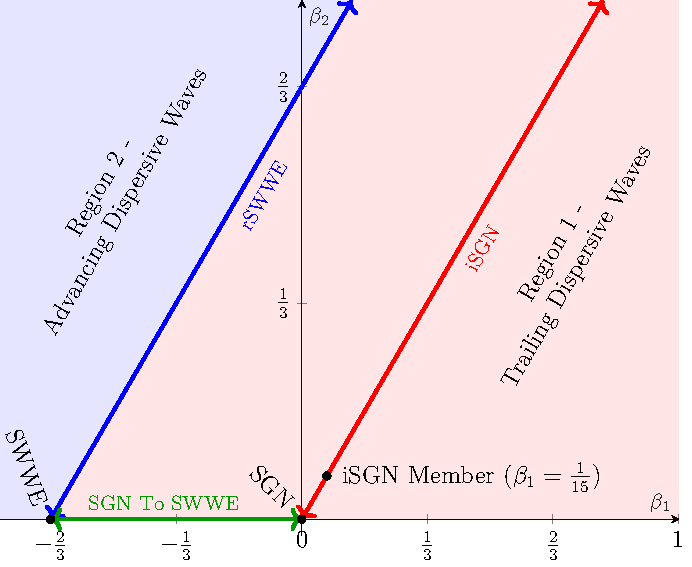
\includegraphics[width=0.4\textwidth]{./Figures/Explanation/BetaPlotAll.pdf}
	\caption{Phase speed regions of gSGN in terms of $\beta_1$ and $\beta_2$ showing important families of equations and particular members of these families.}
	\label{Fig:WaveSpeedReg}
\end{figure}


%-------------------------------------------------
\subsection{Alternative Conservative Form of the gSGN}
%-------------------------------------------------
\citet{Clamond-Dutykh-2018-237} demonstrate a rearrangement of \eqref{eq:gSGNuh} for the rSWWE, in an analogous way to the reformulations of SGN \cite{Hank-etal-2010-2034,Li-2014-169,Zoppou-etal-2017}. The purpose of this reformulation is to remove the mixed spatial-temporal derivative in the flux term, which is difficult to treat numerically. The reformulation works analogously for the gSGN equations as well, and thus an equivalent formulation of \eqref{eq:gSGNuh} can be obtained, giving
\begin{gather*}\label{eq:G_momentum}
\dfrac{\partial G }{\partial t}  + \dfrac{\partial}{\partial x} \left ( uG + \dfrac{gh^2}{2} - \left(\frac{2}{3} +  \beta_1\right) h^3\dfrac{\partial u}{\partial x}\dfrac{\partial u}{\partial x}  - \frac{1}{2} \beta_2 g h^2  \left[h\frac{\partial^2 h}{\partial x^2} + \frac{1}{2}\frac{\partial h}{\partial x}\frac{\partial h}{\partial x}\right]\right ) = 0
\end{gather*}
where the new conserved quantity
\begin{gather*}
G = hu - \frac{1}{2}\left(\frac{2}{3} + \beta_1\right) \dfrac{\partial }{\partial x} \left ( h^3 \dfrac{\partial u}{\partial x} \right ).
\end{gather*}
Using the appropriate substitution of $\beta_1$ values, the conserved variables introduced by \citet{Clamond-Dutykh-2018-237} for the rSWWE as well as for the SGN equations \cite{Hank-etal-2010-2034,Li-2014-169,Zoppou-etal-2017} can be obtained. 

Making this reformulation, provides the equation of mass for the gSGN and an equation in conservation law form for $G$ which is equivalent to the conservation of momentum equations as follows
\begin{subequations}
\begin{gather}
\dfrac{\partial h}{\partial t} + \dfrac{\partial (uh)}{\partial x} = 0
\label{eq:gSGN_Gh}
\end{gather}
\begin{gather}
\dfrac{\partial G }{\partial t}  + \dfrac{\partial}{\partial x} \left ( uG + \dfrac{gh^2}{2} - \frac{2}{3}\left(1 + \frac{3}{2} \beta_1\right) h^3\dfrac{\partial u}{\partial x}\dfrac{\partial u}{\partial x}  - \frac{1}{2} \beta_2 g h^2  \left[h\frac{\partial^2 h}{\partial x^2} + \frac{1}{2}\frac{\partial h}{\partial x}\frac{\partial h}{\partial x}\right]\right ) = 0.
\label{eq:gSGN_GG}
\end{gather}
with
\begin{gather}\label{eq:G_divergent}
G = uh - \frac{1}{3}\left(1 + \frac{3}{2} \beta_1\right) \dfrac{\partial }{\partial x} \left ( h^3 \dfrac{\partial u}{\partial x} \right ).
\end{gather}
\label{eq:gSGN_G}
\end{subequations}
This form of the equations and a bound on the wave speeds, allows \eqref{eq:gSGN_G} to be solved numerically using a combination of finite difference and finite volume methods as performed by \citet{Zoppou-etal-2017} for the SGN.

\section{Numerical Method}
The numerical method proposed for the gSGN, is very similar to methods published for the SGN \cite{Zoppou-etal-2017}. For brevity, only provide a general overview of the method is provided, with highlights of the important differences that need to be made to solve the gSGN instead of the SGN.

\subsection{Overview}
The numerical method for the gSGN equations proceeds very similarly to the SGN equations, space is discretised into cells of fixed width $\Delta x$, and time is partitioned into fixed time steps $\Delta t$. The midpoints of the $j^{th}$ cell are given by $x_j = x_0 + j \Delta x$, while the $n^{th}$ time step is given by $t^n = t^0 + n \Delta t$. Additionally for an arbitrary quantity $q$ the cell average of $q$ in the $j^{th}$ cell at time $t^n$ is defined as 
\[\bar{q}^n_j = \frac{1}{\Delta x} \int_{x_j - \Delta x / 2}^{x_j - \Delta x / 2} q(x,t^n) \; dx.\]
The overview will be using the value of quantities at all cells at a particular time and so $\vecn{q}^n$ is defined to be the vector of $q^n_j$ values and $\bar{\vecn{q}}^n$ to be the vector of $\bar{q}^n_j$ values for all cells in the domain. 

Following, \citet{Zoppou-etal-2017} the gSGN equations can be solved using the method outlined below beginning at a generic $n^{th}$ time step
\begin{enumerate}
	\item Begin with the vectors of cell averages $\bar{\vecn{h}}^n$ and $\bar{\vecn{G}}^n$.
	\item Solve \eqref{eq:G_divergent} with a second-order finite difference method using $\bar{\vecn{h}}^n$ and $\bar{\vecn{G}}^n$ to obtain an approximation to ${\vecn{u}}^n$, which can be written
	\[{A}\left(\bar{\vecn{h}}^n,\bar{\vecn{G}}^n\right) = {\vecn{u}}^n.\]
	\item Solve \eqref{eq:gSGN_Gh} and \eqref{eq:gSGN_GG} using a second-order finite volume method with the approximate Riemann solver of \citet{Kurganov-etal-2001-707} to obtain $\bar{h}^{n+1}_j$ and $\bar{G}^{n+1}_j$ at the next time step, obtaining
	\[{F}\left(\bar{\vecn{h}}^n,\bar{\vecn{G}}^n,{\vecn{u}}^n\right) = \bar{\vecn{h}}^{n+1 },\bar{\vecn{G}}^{n+1}.\]
	\item Combining these steps gives
	\[{E}(\bar{\vecn{h}}^{n},\bar{\vecn{G}}^{n}) = \bar{\vecn{h}}^{n+1 },\bar{\vecn{G}}^{n+1}.\]
	\item However, since ${F}$ is only first order accurate in time steps 1-4 are repeated and then fully second-order approximations to $\bar{\vecn{h}}^{n+1 }$,$\bar{\vecn{G}}^{n+1}$ are obtained using a SSP Runge Kutta method \cite{Gottlieb-etal-2003-89} like so
	\begin{align*}
	{E}(\bar{\vecn{h}}^{n},\bar{\vecn{G}}^{n}) &= \bar{\vecn{h}}^{'},\bar{\vecn{G}}^{'}\\
	{E}(\bar{\vecn{h}}^{'},\bar{\vecn{G}}^{'}) &= \bar{\vecn{h}}^{''},\bar{\vecn{G}}^{''}\\
	\frac{1}{2}\left(\bar{\vecn{h}}^{'} + \bar{\vecn{h}}^{''} \right) = \bar{\vecn{h}}^{n+1 } &\text{  and  }
		\frac{1}{2}\left(\bar{\vecn{G}}^{'} + \bar{\vecn{G}}^{''} \right) = \bar{\vecn{G}}^{n+1 }. 
	\end{align*}
\end{enumerate}

\subsection{Differences}
Although the numerical method to solve the SGN demonstrated by \citet{Zoppou-etal-2017} can be readily adapted to the gSGN, there are some important differences. In particular, the reconstruction of $u$ must be modified to allow discontinuities, additional derivatives must be approximated and the wave speed bounds must be altered. 

\subsubsection{Reconstruction of $u$}
Since the assumption for the SGN that $u$ is continuous across the cells doesn't hold in general for all $\beta$ values, particularly the SWWE pair, the numerical method must be modified. Therefore, the left and right values of $u$ at the cell edge $x_{j+1/2} = x_j + \Delta x /2$,  $u^-_{j+1/2}$ and $u^+_{j+1/2}$  are reconstructed from the $j^{th}$ and $(j+1)^{th}$ cells respectively. These reconstructions are performed like so
\begin{align}
u^+_{j+1/2} &= u_j + \frac{\Delta x}{2} d_j, \\
u^-_{j+1/2} &= u_j - \frac{\Delta x}{2} d_j, \\
d_j &= \text{minmod}\left\lbrace \theta \dfrac{u_{j} - u_{j-1}}{\Delta x}, \dfrac{u_{j+1} - u_{j-1}}{2 \Delta x}, \theta \dfrac{u_{j+1} - u_{j}}{\Delta x} \right \rbrace
\end{align}
where minmod function is defined as follows
\begin{equation}
\text{minmod}\left\lbrace a_0,\dots \right\rbrace = \left \lbrace \begin{array}{l c r}
\min\left\lbrace a_0,\dots \right\rbrace &,& a_i > 0 \text{ for all } i\\
\max\left\lbrace a_0,\dots   \right\rbrace &,& a_i < 0 \text{ for all } i\\
0 &,& \text{otherwise}
\end{array} \right. .
\end{equation}
The $\theta$ parameter is a free parameter between $1$ and $2$, that controls this diffusivity of the reconstruction. When $\theta =1$ the reconstruction is most diffusive, and when $\theta=2$ it is the least diffusive. This method of reconstruction for $u$ at the cell edges makes it consistent with the method to approximate $h$ and $G$ at the cell edges \cite{Zoppou-etal-2017}. 

\subsubsection{Approximations for additional derivatives}
%Make consistent - symmetric, choose approximations that contain the derivatives.
%make them consistent when solutions are smooth, not just smallest, 
The SGN equations only contain the derivative $\partial u / \partial x$ in the flux term, while the gSGN flux term also contains the derivatives $\partial h / \partial x$ and $\partial^2 h / \partial x^2$. These derivatives must be approximated robustly, particularly in the presence of large changes in the primitive quantities. To accomplish this, the minmod function was used to control the size of these derivatives at the cell edges in the following way
\begin{align*}
\left[\dfrac{\partial q}{\partial x} \right]^-_{j+1/2} &= \text{minmod}\left\lbrace \dfrac{2 q_j - 3 q_{j-1} + q_{j-2}}{\Delta x} , \dfrac{q_{j+1} - q_j}{\Delta x} \right\rbrace , \\
\left[\dfrac{\partial q}{\partial x} \right]^+_{j+1/2} &= \text{minmod}\left\lbrace \dfrac{-2 q_{j+1} - 3 q_{j+2} + q_{j+3}}{\Delta x} , \dfrac{q_{j+1} - q_j}{\Delta x} \right\rbrace \\
\left[\dfrac{\partial^2 q}{\partial x^2} \right]^-_{j+1/2} &= \text{minmod}\left\lbrace \dfrac{5q_j - 13 q_{j-1} + 11q_{j-2} - 3 q_{j-3}}{2\Delta x^2}, \dfrac{3q_{j+1} -7q_j +5q_{j-1} - q_{j-2} }{2\Delta x^2}  , \dfrac{q_{j+2} - q_{j+1} - q_j + q_{j-1}}{2 \Delta x^2} \right\rbrace , \\
\left[\dfrac{\partial^2 q}{\partial x^2} \right]^+_{j+1/2} &= \text{minmod}\left\lbrace \dfrac{3q_j - 7 q_{j+1} + 5 q_{j+2} - 3 q_{j+3}}{2\Delta x^2}, \dfrac{5q_{j+1} - 13q_{j+2} + 11q_{j+ 3} - 3 q_{j+4} }{2\Delta x^2}  , \dfrac{q_{j+2} - q_{j+1} - q_j + q_{j-1}}{2 \Delta x^2} \right\rbrace.
\end{align*}

The limiting performed here is comparing the various second-order approximations to the derivatives, using the values in the appropriate neighbouring cells. When these approximations have the same sign, it chooses the one with the lowest value, otherwise it is zero. This works to improve the robustness of the scheme, since the method always uses the smallest approximation in the first case, and in the second case the derivative is removed as the solution is no longer smooth or the derivative is very close to zero anyway. 

\subsubsection{Wave speed bounds}
Since the expressions for the bounds on the wave speeds of the gSGN equations depend on the $\beta$ values whereas the equivalent wave speed bounds for the SGN equations were derived for one pair of $\beta$ values, the calculation of the wave speed bounded must be updated accordingly. In particular,the two wave speed bounds for waves emanating from cell edge $x_{j} + \Delta x /2$ which were $a^\pm_{j+1/2}$ are calculated in the following way
\begin{align}
a^+_{j+1/2} &= \max\left\lbrace 0, \: u^+_{j+1/2} + \sqrt{\dfrac{\beta_2}{\frac{2}{3} + \beta_1}} \sqrt{g h^-_{j+1/2}}, \: u^-_{j+1/2} + \sqrt{\dfrac{\beta_2}{\frac{2}{3} + \beta_1}}\sqrt{g h^-_{j+1/2}} \right\rbrace, \\
a^-_{j+1/2} &= \min\left\lbrace 0,\: u^+_{j+1/2} - \sqrt{\dfrac{\beta_2}{\frac{2}{3} + \beta_1}}\sqrt{g h^-_{j+1/2}},\: u^-_{j+1/2} - \sqrt{\dfrac{\beta_2}{\frac{2}{3} + \beta_1}}\sqrt{g h^-_{j+1/2}} \right\rbrace.
\end{align}


\section{Validation}
The numerical method described above is validated using analytic solutions for particular $\beta$ values that correspond to the SGN equations and the SWWE and a forced solution. Together these tests demonstrate the ability of the method to reproduce analytic solutions to important members of the gSGN family, as well as solve the gSGN for any pair of $\beta$ values that admit wave speed bounds.

The accuracy of the numerical method will be measured using the distance between the numerical solution and the equivalent analytic or forced solution using the $L_2$ norm. While the conservation properties of the numerical method will be measured by numerically approximating the energy in the initial conditions and the numerical solution and comparing them using a measure called $C_1$.

For a quantity $q$ with a vector of its analytic or forced solution at the cell midpoints $\vecn{q}$ and the numerical solution at the cell midpoints $\vecn{q}^*$, the discrete $L_2$ norm is
\begin{equation}
\label{eqn:Conv_Error}
L_2\left(\vecn{q},\vecn{q}^*\right) = \sqrt{ \dfrac{\sum_{j = 0}  \left[q_j^2 - \left(q^*_j\right)^2 \right]}{\sum_{j = 0}  \left[q_j^2 \right]}}
\end{equation}
where the time-step superscripts were suppressed for simplicity.

For a quantity $q$ with a vector of its values at the $n^{th}$ time step $\vecn{q}^n$, the total amount of the quantity is approximated by $C(\vecn{q}^n)$. The method for this is the same as the method described by \citet{Zoppou-etal-2017}, which has a higher order of accuracy than the numerical method it is measuring. Using the numerical approximation to the total amounts, the conservation error is obtained in the following way
\begin{equation}
\label{eqn:Cons_Error}
C_1\left(\vecn{q}^0,\vecn{q}^n\right) = \left \lbrace \begin{array}{l c r}
\dfrac{\left | C(\vecn{q}^0) - C(\vecn{q}^n) \right |}{\left| C(\vecn{q}^0) \right|}&,& \left| C(\vecn{q}^0) \right| > 0 \T \\
\left | C(\vecn{q}^0) - C(\vecn{q}^n) \right |&,& \left| C(\vecn{q}^0) \right| = 0 
\end{array} \right. .
\end{equation}

\begin{itemize}
	\item Analytic solutions - we recover them (conservation and norm)
	\item Forced solutions - our numerical method can handle any combination of beta values, all terms are approximated with correct order of accuracy. Limiters on gradients off. 
\end{itemize}

\subsection{Analytic Solutions}
The analytic solutions used to validate the numerical method, are the soliton solution of the SGN equations and the dam-break solution of the SWWE. The soliton solution is a smooth travelling wave solution, that assesses the balance of the non-linear and dispersive terms in the gSGN equations. Whereas the dam-break solution of the SWWE demonstrates the robustness of the method in the presence of steep gradients. The soliton solution used in this paper, is the same as the soliton solution used for validation by \citet{Pitt-2019}, allowing for a comparison of this gSGN solver to the more specialised SGN solvers described in that paper. 

\subsubsection{Serre Equations ($\beta_1=\beta_2 =0$) - Solitary Travelling Wave Solution}
When $\beta_1 = \beta_2 = 0$ the gSGN are equivalent to the SGN equations which admit the following travelling wave solution
\begin{subequations}
	\begin{equation}
	h(x,t) = a_0 + a_1 \text{sech}^2\left( \kappa (x - ct) \right),
	\end{equation}
	\begin{equation}
	u(x,t) = c \left( 1- \dfrac{a_0}{h(x,t)} \right),
	\end{equation}
	where
	\begin{equation}
	\kappa = \dfrac{\sqrt{3a_1}}{2a_0 \sqrt{a_0 + a_1}}
	\end{equation}
	and
	\begin{equation}
	c = \sqrt{g\left(a_0 + a_1\right)}.
	\end{equation}
\end{subequations}

This travelling wave solution is maintained due to a balance between the dispersive terms and the non-linear terms in the momentum equation \eqref{eq:G_momentum}. Validating the numerical solutions for the gSGN solver using this solution tests the balance between these terms in \eqref{eq:G_momentum}, and allows us to verify the method's conservation of energy as the solution is smooth. To enable a comparison between the numerical method and the SGN solver of \cite{Zoppou-etal-2017} the chosen soliton parameters were $a_0 = 1$ and $a_1 = 0.7$ and the acceleration due to gravity at the earth surface, $g = 9.81 m^2/s$ was used.

The numerical solution was solved over the domain $\left[-200,200\right]$ from $t=0s$ until $t=30s$. To ensure that the SGN solution is recovered, $\beta_1 = \beta_2=0$. The spatial resolution was varied like so $\Delta x = 400 / (100 \times 2^{l})$, where $l$ was increased. To satisfy the Courant-Friedrichs-Lewy (CFL) condition \cite{Lax-Richtmyer-1956-267} the time step width $\Delta t = \Delta x  / \left( 2 \sqrt{g \left(a_0 + a_1\right)}\right)$ \cite{Pitt-2019} was chosen. The limiting parameter $\theta$ was set to $\theta = 1.2$, matching the numerical experiments performed by \citet{Pitt-2019}.

Example numerical solutions for $h$, $u$ and $G$ with $\Delta x = 400 / (100 \times 2^{6}) \simeq 0.06m$ are plotted in Figure \ref{Fig:Sol_Ex}. These examples demonstrate that the numerical solutions well reproduced the analytic solutions.
%
\begin{figure}
	\centering
	\begin{subfigure}{0.32\textwidth}
		\centering
		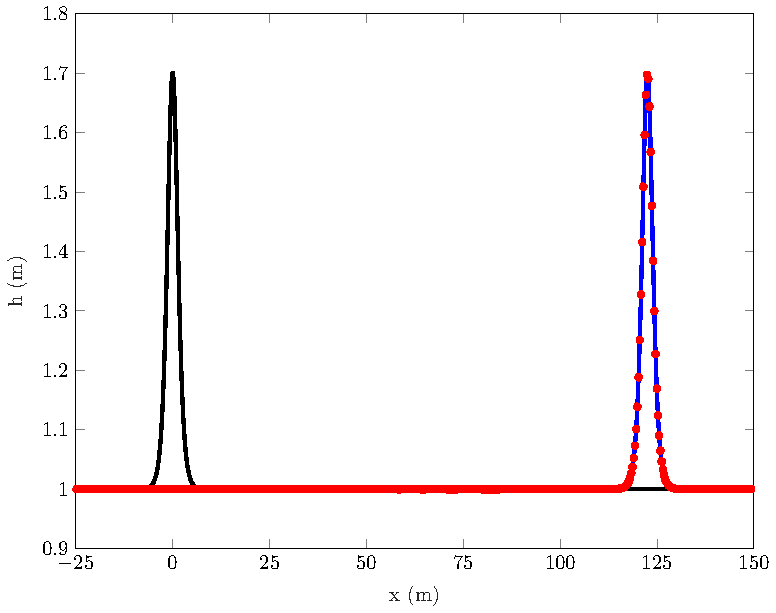
\includegraphics[width=\textwidth]{./Figures/Simulations/Validation/Serre/h.pdf}
		\caption{$h$}
	\end{subfigure}
	\begin{subfigure}{0.32\textwidth}
		\centering
		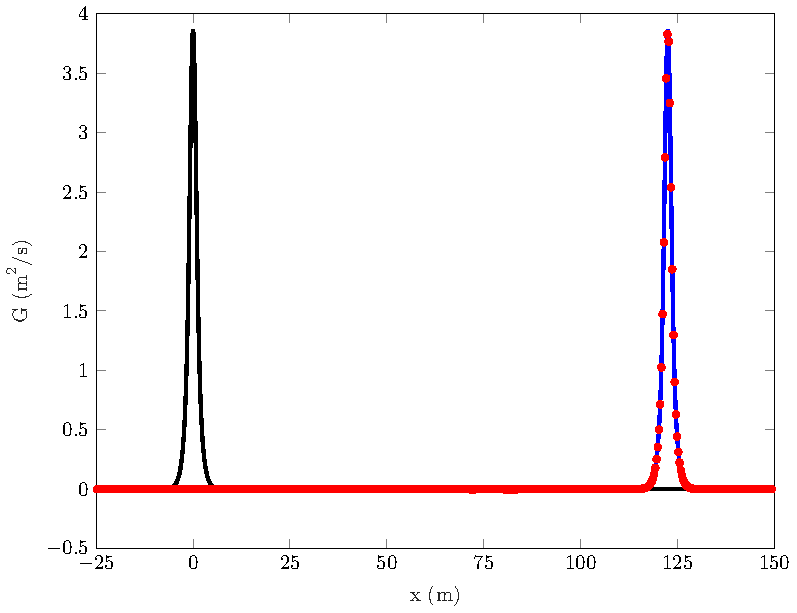
\includegraphics[width=\textwidth]{./Figures/Simulations/Validation/Serre/G.pdf}
		\caption{$G$}
	\end{subfigure}
	\begin{subfigure}{0.32\textwidth}
		\centering
		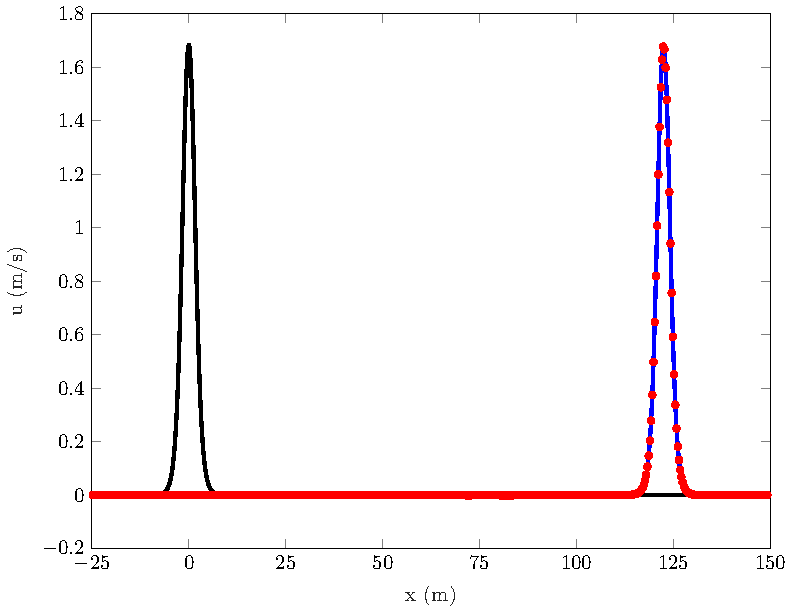
\includegraphics[width=\textwidth]{./Figures/Simulations/Validation/Serre/u.pdf}
		\caption{$u$}
	\end{subfigure}
	\caption{Plot of comparing initial (\solidrule), analytic solution ({\color{blue}\solidrule}), and numerical solution with $\Delta x \approx 0.06m$ (\tikzcircle{red}) at $t = 30s$.}
	\label{Fig:Sol_Ex}
\end{figure}

A comparison of many numerical solutions with varying $\Delta x$ are given in Figure \ref{Fig:Sol_Comp} for both the convergence and conservation measures. These plots demonstrate that the scheme obtains second-order convergence for all quantities of interest, after $\Delta x$ becomes small enough to properly represent the initial conditions. 
%
\begin{figure}
	\centering
	\begin{subfigure}{0.49\textwidth}
		\centering
		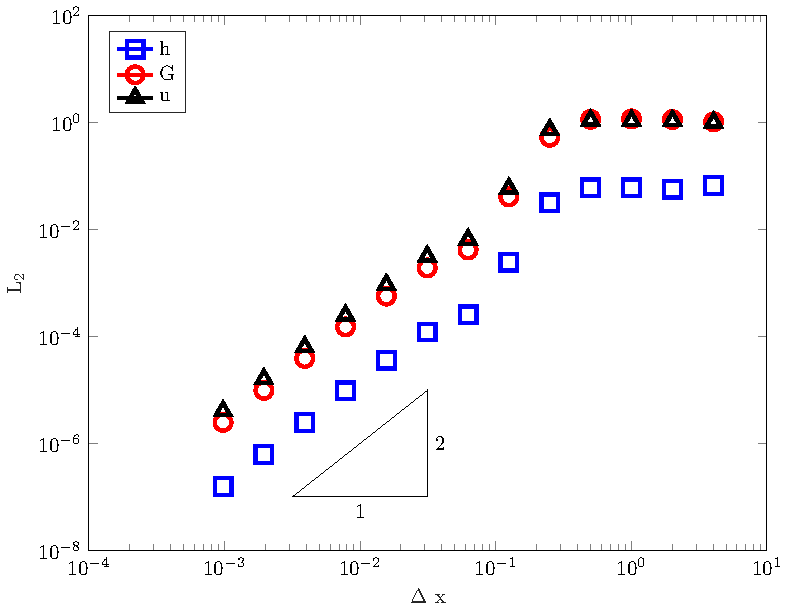
\includegraphics[width=\textwidth]{./Figures/Simulations/Validation/Serre/NormResults.pdf}
		\caption{$L_2$ with $u$ (\trianglet{black})}
		\label{Fig:Sol_Comp_Conv}
	\end{subfigure}
	\begin{subfigure}{0.49\textwidth}
		\centering
		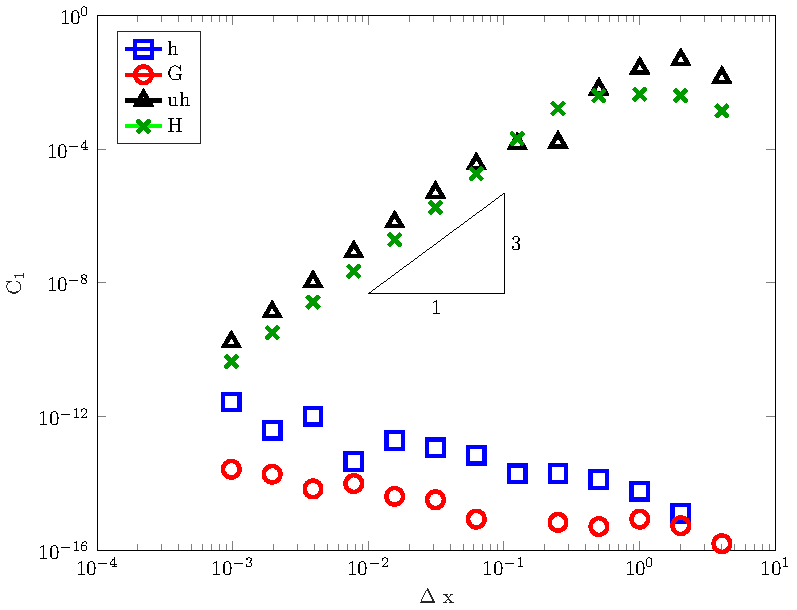
\includegraphics[width=\textwidth]{./Figures/Simulations/Validation/Serre/EnergyResults.pdf}
		\caption{$C_1$ with $uh$ (\trianglet{black})}
		\label{Fig:Sol_Comp_Cons}
	\end{subfigure}
	\caption{Convergence and conservation plots for $h$ (\squaret{blue}) , $G$ (\circlet{red}) and $\mathcal{H}$ (\crosst{green!60!black}) as $\Delta x$ varies.}
	\label{Fig:Sol_Comp}
\end{figure}
%
The conservation plot in Figure \ref{Fig:Sol_Comp_Conv} demonstrates that due to the use of the finite volume method $h$ and $G$ are conserved up to round-off error, which increases as $\Delta x$ increases. The conservation of $uh$ and $\mathcal{H}$ whilst not being at round-off error does reduce at a rate better than second-order and so the scheme possesses good convergence and conservation properties. These results agree well with the numerical solutions of \citet{Pitt-2019}, who compared various numerical methods. 

\subsubsection{SWWE ( $\beta_1= -\frac{2}{3}$ and $ \beta_2 =0$ ) - Dam-break Solution }
When $\beta_1= -\frac{2}{3}$ and $ \beta_2 =0$ the gSGN equations reduce to the SWWE which have an analytic solution to the dam-break problem given by the initial conditions
\begin{align}
h(x,0) & = \left\lbrace \begin{array}{c c}
h_0 & x < 0\\
h_1 & x \ge 0
\end{array} \right.  \\
u(x,0) &= 0 \\
G(x,0) &= 0.
\end{align}

The solution to the dam-break problem is given by
\begin{align}
h(x,t) &= \left \lbrace \begin{array}{l c r}
h_0 &,& x \le -t\sqrt{g h_0} \\
\frac{4}{9g} \left(\sqrt{gh_0} - \frac{x}{2t}\right)^2 &,&  -t\sqrt{g h_0} < x \le t \left(u_2 - \sqrt{g h_2}\right)  \\
h_2 &,&  t \left(u_2 - \sqrt{g h_2}\right) < x \le t S_2  \\
h_1 &,&   t S_2 \le x \\
\end{array} \right.  \\
u(x,t) &= \left \lbrace \begin{array}{l c r}
0 &,& x \le -t\sqrt{g h_0} \\
\frac{2}{3} \left(\sqrt{gh_0} + \frac{x}{t}\right) &,&  -t\sqrt{g h_0} < x \le t \left(u_2 - \sqrt{g h_2}\right)  \\
u_2 &,&  t \left(u_2 - \sqrt{g h_2}\right) < x \le t S_2  \\
0 &,&   t S_2 \le x \\
\end{array} \right. .
\end{align}
%
The constant state values $h_2$ and $u_2$ and the shock speed $S_2$ can be calculated for any initial conditions by solving
\begin{align}
\label{eq:SWWEMiddleState}
h_2 &= \dfrac{h_0}{2} \left(  \sqrt{1 + 8 \left( \dfrac{2 h_2}{h_2 - h_0} \left(\dfrac{\sqrt{gh_1} - \sqrt{gh_2}}{\sqrt{gh_0}}\right)\right)^2 } - 1 \right) \\
u_2 &= 2\left(\sqrt{gh_1} - \sqrt{gh_2} \right),\\
S_2 &= \dfrac{2 h_2}{h_2 - h_1}\left(\sqrt{gh_0} - \sqrt{gh_2} \right).
\end{align}

The initial conditions as well as the analytic solution are discontinuous. Due to the discontinuities the solutions to the initial conditions are not unique, as solving any pair of the 3 conservation equations \eqref{eq:gSGN}, gives solutions with similar structures but different constant values. The solution presented above is solution of the mass and momentum equations, as these equations are the basis of the numerical method.

A number of numerical experiments were run for the dam-break problem with $h_0 = 2m$ and $h_1 = 1m$. The domain of the solution was $\left[-250,250\right]$ with a final time of $t=35s$.  The spatial resolution was varied like so $\Delta x = 500 / (1000 \times 2^{l})$, while to satisfy the CFL condition \cite{Lax-Richtmyer-1956-267} the time step width $\Delta t = \Delta x  / \left( 2 \sqrt{g h_0}\right)$ was used. The limiting parameter $\theta$ was set to be $\theta = 1.2$ and the acceleration due to gravity $g = 9.81 m^2/s$ was used. 

Example numerical solutions and analytic solutions for $h$, $G$ and $u$ at the final time with the spatial resolution $\Delta x = 500 / (1000 \times 2^{4})$ are plotted in Figure \ref{Fig:DB_Ex}. These figures demonstrate that the method is robust in the presence of steep gradients and appropriately reproduces the broad structure of the analytic solution. 
%
\begin{figure}
	\centering
	\begin{subfigure}{0.32\textwidth}
		\centering
		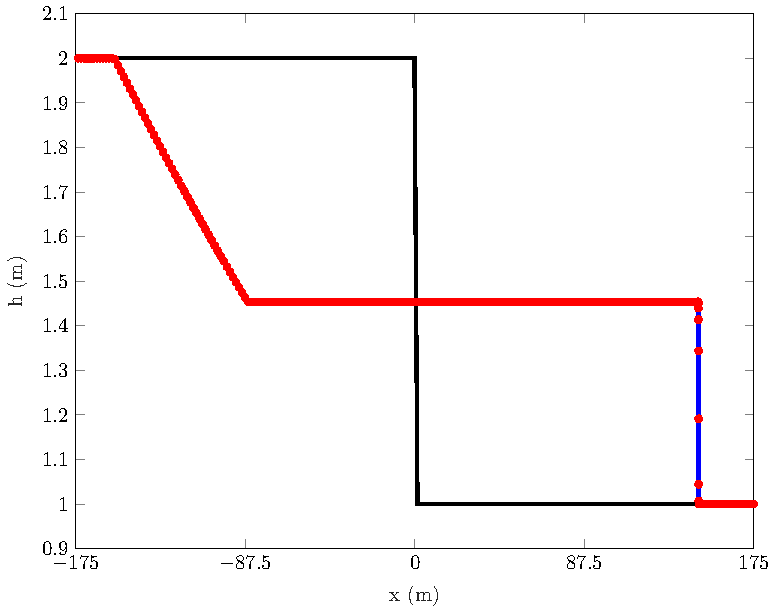
\includegraphics[width=\textwidth]{./Figures/Simulations/Validation/DBSWWE/h.pdf}
		\caption{$h$}
	\end{subfigure}
	\begin{subfigure}{0.32\textwidth}
		\centering
		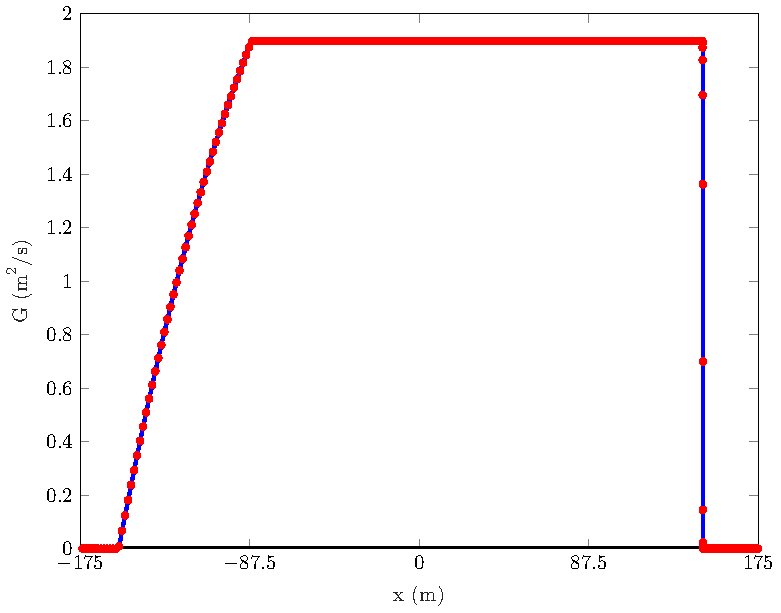
\includegraphics[width=\textwidth]{./Figures/Simulations/Validation/DBSWWE/G.pdf}
		\caption{$G = uh$}
	\end{subfigure}
	\begin{subfigure}{0.32\textwidth}
		\centering
		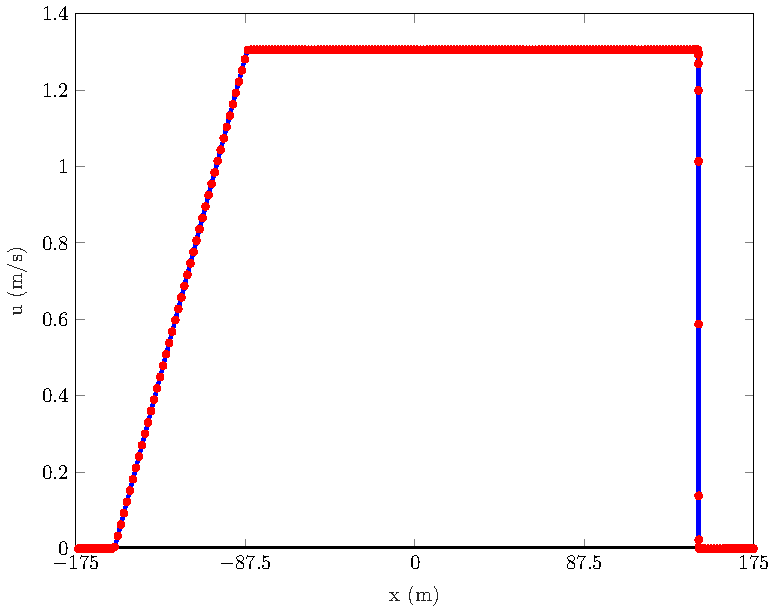
\includegraphics[width=\textwidth]{./Figures/Simulations/Validation/DBSWWE/u.pdf}
		\caption{$u$}
	\end{subfigure}
	\caption{Comparison of initial (\solidrule), analytic solution ({\color{blue}\solidrule}), and numerical solution with $\Delta x \approx 0.03m$ (\tikzcircle{red}) at  $t=35s$.}
	\label{Fig:DB_Ex}
\end{figure}

The central difficulty of reproducing the analytic solutions for the dam-break problem, is observed around only a few critical locations; the top of the rarefaction fan, the bottom of the rarefaction fan and the shock front. Figure \ref{Fig:Conv_Ex} demonstrates the convergence of the solutions for $h$ as $\Delta x$ changes for the top of the rarefaction fan and the shock front. 
%
\begin{figure}
	\centering
	\begin{subfigure}{0.45\textwidth}
		\centering
		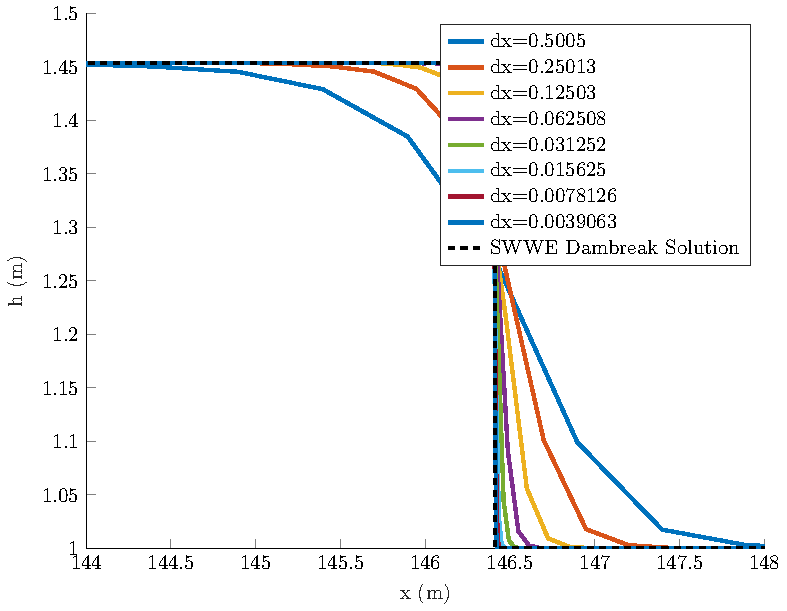
\includegraphics[width=\textwidth]{./Figures/Simulations/Validation/DBSWWE/hFront.pdf}
		\caption{Shock front}
	\end{subfigure}
	\begin{subfigure}{0.45\textwidth}
		\centering
		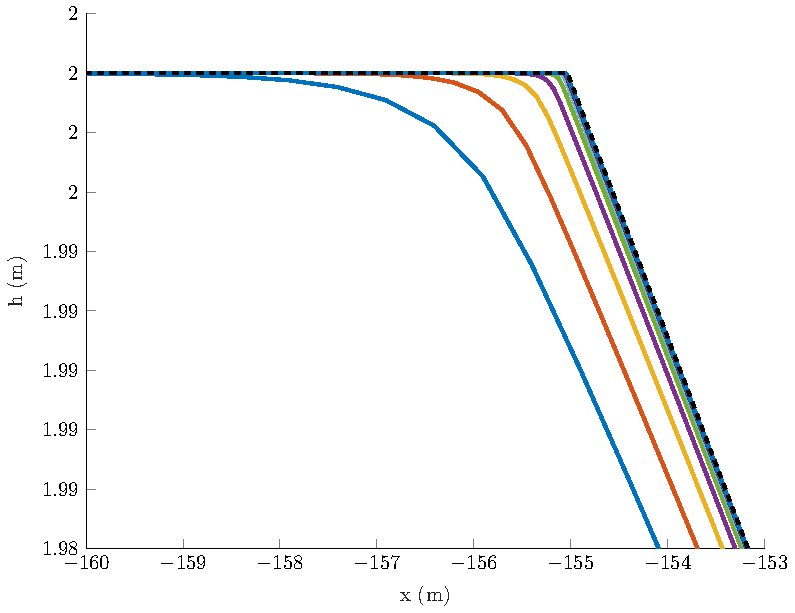
\includegraphics[width=\textwidth]{./Figures/Simulations/Validation/DBSWWE/hRFTop.pdf}
		\caption{Top of rarefaction fan}
	\end{subfigure}
	\caption{Plots of $h$ at $t=35s$ for the smooth dam-break problem around important locations with $\Delta x = 2^{-1}$ ({\color{mycolor1}\solidrule}), $2^{-2}$ ({\color{mycolor2}\solidrule}), $2^{-3}$ ({\color{mycolor3}\solidrule}), $2^{-4}$ ({\color{mycolor4}\solidrule}), $2^{-5}$ ({\color{mycolor5}\solidrule}), $2^{-6}$ ({\color{mycolor6}\solidrule}), $2^{-7}$ ({\color{mycolor7}\solidrule}), $2^{-8}$ ({\color{mycolor1}\solidrule}) and the analytic solution ({\dashedrule}) of the SWWE to the corresponding dam-break problem.}
	\label{Fig:Conv_Ex}
\end{figure}
%
Figure \ref{Fig:Conv_Ex} demonstrates that as $\Delta x$ decreases tje numerical solutions are converging to better resolve these critical locations. The behaviour of the bottom of the rarefaction fan is very similar to the top, and the behaviour of the solutions for $u$ and $G$ is similar, and so has been omitted. The convergence of the numerical methods is difficult to measure since the solutions are discontinuous, and so this more visual approach is used. In the presence of discontinuities the method is no longer expected to be fully second-order accurate, due to the use of the limiters, even so the method still possesses good convergence properties in the presence of the discontinuities.

Figure \ref{Fig:DB_Cons} shows the conservation properties of the numerical solutions as $\Delta x$ decreases. The conservation of $h$ and $G=uh$ is at round-off error and thus the error gets larger as $\Delta x$ decreases and the number of calculations increases. The conservation of $u$ is now only first-order, while the conservation of $\mathcal{E}$ doesn't improve as $\Delta x$ decreases. The drop in order for conservation of $u$ is due to the use of limiters which whilst making the numerical method total variation diminishing \cite{LeVeque-2002} and more robust, also result in the reconstruction becoming first-order near discontinuities. The lack of improvement in conservation of $\mathcal{E}$ is because the solutions are not sufficiently smooth, and thus do not satisfy all conservation equations \eqref{eq:gSGN} simultaneously \cite{Pu-2018-1361}. The loss of conservation in $\mathcal{H}$ is also a feature of the analytic solution as can be seen in Figure \ref{Fig:DB_Energy} which plots the total amount of energy over time for numerical and the analytic solutions. 
%
%Remove uh and energy, since energy dissipated anyway
\begin{figure}
	\centering
	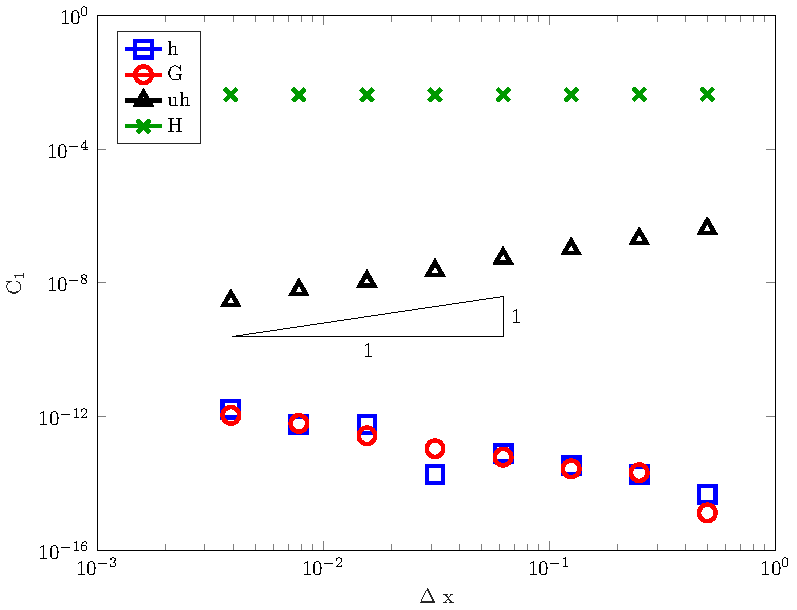
\includegraphics[width=0.5\textwidth]{./Figures/Simulations/Validation/DBSWWE/EnergyResults.pdf}
	\caption{Conservation Plots  $h$ (\squaret{blue}) , $G$ (\circlet{red}), $uh$ (\trianglet{black}), $\mathcal{H}$ \crosst{green!60!black}.}
	\label{Fig:DB_Cons}
\end{figure}
%
\begin{figure}
	\centering
	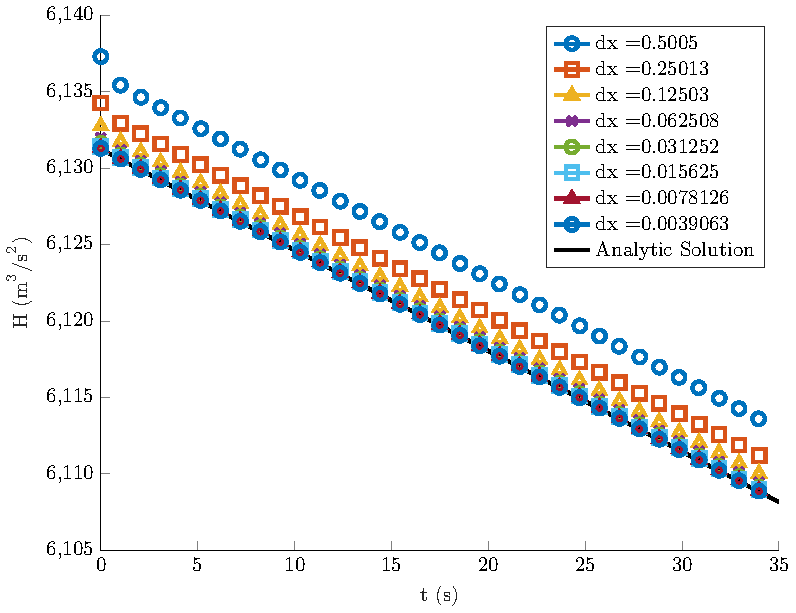
\includegraphics[width=0.49\textwidth]{./Figures/Simulations/Validation/DBSWWE/EnergyOverTime.pdf}
	\caption{Plot of total energy $\mathcal{H}$ for numerical solutions over time with $\Delta x = 2^{-1}$ ({\color{mycolor1}\circlet{}}), $2^{-2}$ ({\color{mycolor2}\squaret{}}), $2^{-3}$ ({\color{mycolor3}\trianglet{}}), $2^{-4}$ ({\color{mycolor4}\crosst{}}), $2^{-5}$ ({\color{mycolor5}\circlet{}}), $2^{-6}$ ({\color{mycolor6}\squaret{}}), $2^{-7}$ ({\color{mycolor7}\trianglet{}}), $2^{-8}$ ({\color{mycolor1}\crosst{}}) and the analytic solution ({\solidrule}) of the SWWE to the corresponding dam-break problem..}
	\label{Fig:DB_Energy}
\end{figure}

These results demonstrate that the analytic solution of the SWWE has been accurately reproduced by the numerical method. 

\subsection{Forced Solutions}
To demonstrate the validity and versatility of the method to solve the gSGN for any $\beta$ values, forced solutions were used. To generate a forced solution the forced gSGN equations are considered
\begin{subequations}
	\begin{gather}
	\dfrac{\partial h}{\partial t} + \dfrac{\partial (uh)}{\partial x} = \dfrac{\partial h^*}{\partial t} + \dfrac{\partial (u^*h^*)}{\partial x} 
	\label{eq:gSGN_Gh_Forced}
	\end{gather}
	\begin{multline}
	\dfrac{\partial G }{\partial t}  + \dfrac{\partial}{\partial x} \left ( uG + \dfrac{gh^2}{2} - \frac{2}{3}\left(1 + \frac{3}{2} \beta_1\right) h^3\dfrac{\partial u}{\partial x}\dfrac{\partial u}{\partial x}  - \frac{1}{2} \beta_2 g h^2  \left[h\frac{\partial^2 h}{\partial x^2} + \frac{1}{2}\frac{\partial h}{\partial x}\frac{\partial h}{\partial x}\right]\right ) = \\ \dfrac{\partial G^* }{\partial t}  + \dfrac{\partial}{\partial x} \left ( u^*G^* + \dfrac{g\left(h^*\right)^2}{2} - \frac{2}{3}\left(1 + \frac{3}{2} \beta_1\right) \left(h^*\right)^3\dfrac{\partial u^*}{\partial x}\dfrac{\partial u^*}{\partial x}  - \frac{1}{2} \beta_2 g \left(h^*\right)^2  \left[h^*\frac{\partial^2 h^*}{\partial x^2} + \frac{1}{2}\frac{\partial h^*}{\partial x}\frac{\partial h^*}{\partial x}\right]\right ).
	\label{eq:gSGN_GG_Forced}
	\end{multline}
	\label{eq:gSGN_Forced}
\end{subequations}
The forced gSGN admit the solutions $h^*$, $u^*$ and $G^*$ assuming $G^*$ appropriately satisfies \eqref{eq:G_divergent}. Since these equations are satisfied for any chosen $h^*$, $u^*$ and $G^*$ and any $\beta$ values, forced solutions can be used to verify the method for a large class of problems. Since the left hand-side of these modified equations are approximated by the numerical method, by combining the numerical method with the analytic expressions for the right hand-side, produces a method that approximates the forced gSGN equation with the same convergence properties as the underlying numerical method for the gSGN equations. 

Since $h^*$, $u^*$ and $G^*$ are arbitrary any desires solution can be generated and used to test the convergence properties for situations for which no known analytic solution to the equations exist. Of particular in this paper are solutions where the $\beta$ values are not equivalent to well studied equations and thus have no known analytic solutions exist, and where all the terms in the equations are non-zero, and thus must be approximated accurately. 

To accomplish these goals the following forced solutions
\begin{subequations}
	\begin{equation}
	h^*(x,t) = a_0 + a_1 \exp\left( \dfrac{\left(x - a_2 t\right)^2}{2 a_3} \right)
	\end{equation}
	\begin{equation}
	u^*(x,t) = a_4 \exp\left( \dfrac{\left(x - a_2 t\right)^2}{2 a_3} \right)
	\end{equation}
	\begin{align}
	\beta_1(x,t) &= a_6 \\
	\beta_2(x,t) &= a_7
	\end{align}
\end{subequations}
where $G^*$ is given by \eqref{eq:G_divergent}, were used. These forced solutions describe Gaussian bumps in $h$ and $u$ that travel at a constant speed $a_2$. The particular parameter values $a_0=1$, $a_1=0.5$, $a_3=20$, $a_4=0.3$, $a_6 = 1$ and $a_7=2$ were chosen in this investigation. Note that using these values, all terms in \eqref{eq:gSGN_G} are non-zero, and thus must be accurately approximated by the numerical method to reproduce the forced solution.

The numerical solutions were produced over the domain $\left[-100,100\right]$ with a final time of $t=10$. The spatial resolution was varied like so $\Delta x = 200 / (100 \times 2^{l})$, while the CFL condition was satisfied by setting $\Delta t = \Delta x  / \left( 2 \left[a_4 + a_2+ \sqrt{g \left(a_0 + a_1\right)}\right] \right)$. The acceleration due to gravity $g=9.81m^2/s$ and the limiting parameter $\theta = 1.2$ was used.

Figure \ref{Fig:FS_Ex} shows example numerical solutions at the final time for $h$, $G$ and $u$ with $\Delta x = 200 / (100 \times 2^{6}) \approx 0.03$. These example solutions demonstrate that the numerical method is able to reproduce the forced solution well.
%
\begin{figure}
	\centering
	\begin{subfigure}{0.32\textwidth}
		\centering
		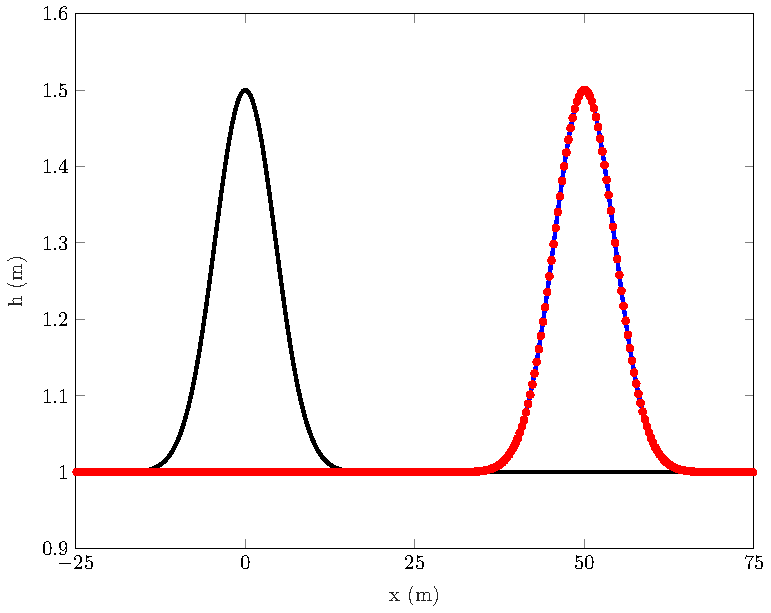
\includegraphics[width=\textwidth]{./Figures/Simulations/Validation/Forced/h.pdf}
		\caption{$h$}
	\end{subfigure}
	\begin{subfigure}{0.32\textwidth}
		\centering
		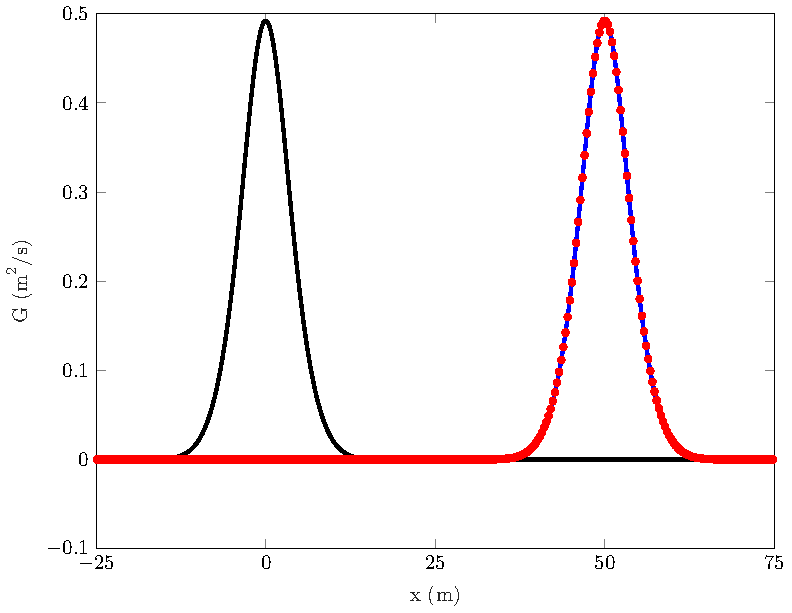
\includegraphics[width=\textwidth]{./Figures/Simulations/Validation/Forced/G.pdf}
		\caption{$G$}
	\end{subfigure}
	\begin{subfigure}{0.32\textwidth}
		\centering
		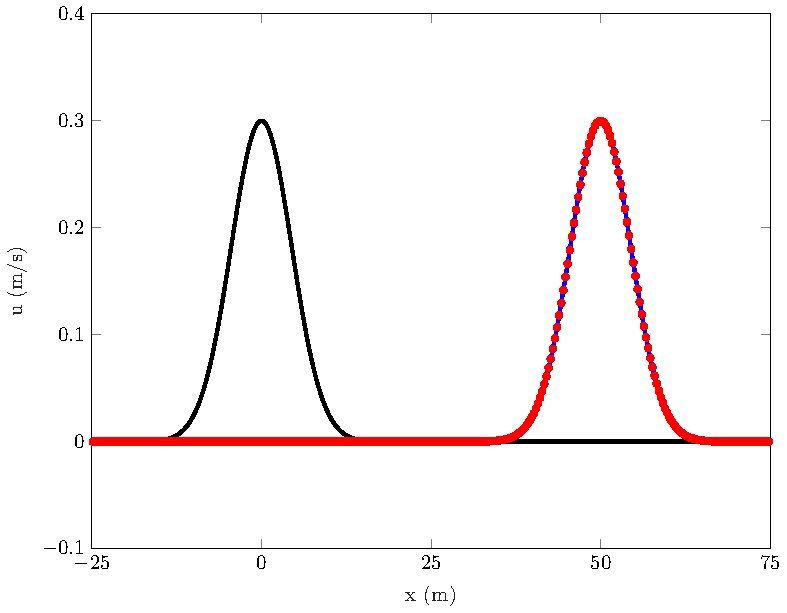
\includegraphics[width=\textwidth]{./Figures/Simulations/Validation/Forced/u.pdf}
		\caption{$u$}
	\end{subfigure}
	\caption{Example plots Initial (\solidrule), analytic solution ({\color{blue}\solidrule}), and numerical solution with $\Delta x \approx 0.03m$ (\tikzcircle{red}).}
	\label{Fig:FS_Ex}
\end{figure}

Figure \ref{Fig:FS_Conv} demonstrates the convergence of the numerical scheme as $\Delta x$ decreases. All quantities of interest are converging at the expected second-order. Since the RHS is given analytically, the observed error is caused by the numerical method. Therefore, these results demonstrate that the scheme is second-order for all terms in gSGN equations. Unfortunately, to be able to accurately reproduce the forced solutions the limiting on the derivatives had to be removed. This made the derivative approximations consistent, and importantly didn't restrict the derivatives at the top of the Gaussian bumps. Thus the forced solutions only validate the method without derivative limiting for all $\beta$ values. However, given that the limiting is only comparing derivative approximations of the same order and the above analytic solutions, the numerical method is well validated.
%
\begin{figure}
	\centering
	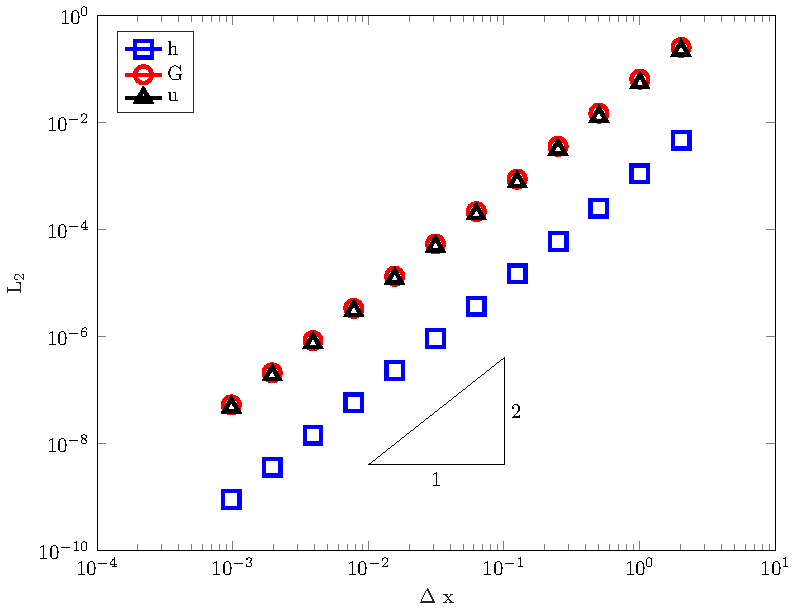
\includegraphics[width=0.49\textwidth]{./Figures/Simulations/Validation/Forced/NormResults.pdf}
	\caption{Convergence plot of $h$ (\squaret{blue}) , $G$ (\circlet{red}), $u$ (\trianglet{black}) for the forced solutions for various $\Delta x$ values.}
	\label{Fig:FS_Conv}
\end{figure}

\section{Smooth Dam-break Study}
Now that the numerical method has been validated for all $\beta$ values above using analytic and forced solutions, this paper will now use the well validated numerical method to embark on a numerical study comparing equations within subfamilies of the gSGN family. The aim of this investigation is to observe the changes in dispersive wave trains and to observe the behaviour of the equations in the presence of steep gradients, particularly for the rSWWE family. 

Both of the aims of this study can be met by comparing numerical solutions to the smooth dam-break problems studied by \citet{Pitt-2018-61} for the SGN defined by the following initial conditions 
\begin{align}
h(x,0) & = h_0 + \dfrac{h_1 - h_0}{2} \left(1 + \tanh\left(\dfrac{x}{\alpha}\right)\right)  \\
u(x,0) &= 0 \\
G(x,0) &= 0.
\end{align}
This family of equations represent a smooth approximation to the dam-break problem initial conditions solved above for the SWWE. This family of initial conditions achieves the aims of the investigation since as shown by \citet{Pitt-2018-61}, due to the steepness in the initial conditions the dispersive wave train that develops extends into very large wave numbers $k$. While this family of initial conditions provides insight into the behaviour of these equations in the presence of steep gradients, particularly when $\alpha$ is small. 

In the rest of the paper the smoothed dam-break problem with $h_0=2$, $h_1 = 1$ and $\alpha = 0.1$ was studied. The spatial domain was $\left[-250,250\right]$ with a final time of $t=35s$. The spatial resolution $\Delta x = 500 / (1000 \times 2^{6}) \simeq 0.007$ was used with the CFL condition satisfied by setting $\Delta t = \Delta x / \left(2 \sqrt{g h_0}\right)$. The acceleration due to gravity $g = 9.81$ and the limiting parameter $\theta = 1.2$ were used.

The particular smoothed dam-break problem was chosen because $\alpha$ is small enough that the high wave-numbers in the dispersive wave-train can be observed \cite{Pitt-2018-61}. The dam-break heights are similar to previous explorations of this initial condition problem for the SGN equations \cite{Clamond-Dutykh-2018-237,Pitt-2018-61,Hank-etal-2010-2034}, although as aspect ratios change there can be significant differences in the structure of the observed dispersive wave train \cite{Zoppou-2014}. Of particular note are the dispersive wave trains corresponding to high Froude number flows, and those for which the downstream depth is close to $0$, which are not studied here for brevity. 

The particular spatial resolution was sufficiently small to properly resolve the structure for our purposes \cite{Pitt-2018-61}, although as demonstrated in the literature such problems are difficult to accurately resolve. However, since this work's primary purpose is to observe the larger patterns and behaviours, the numerical solutions in this study are sufficiently well resolved. 

\subsection{Regularised SWWE Family ($\beta_2 = \frac{2}{3} + \beta_1$)}
The first family of equations of interest is the rSWWE family, these were derived by \citet{Clamond-Dutykh-2018-237}. The primary purpose of these equations were to generate a set of equations that produces regularised solutions to the SWWE. The regularisation is maintained by a balance between the dispersive terms and the regularisation terms in \eqref{eq:G_momentum}, such that the dispersive relation \eqref{eq:DispRelgSGN} reduces to the dispersion relation of the SWWE. A significant benefit of this would be that since solutions are smooth they will be unique and thus satisfy all three conservation equations \eqref{eq:gSGNE} simultaneously. Additionally, if the solutions remain smooth then numerical methods that assume the solution are smooth can be employed to solve them.

Unfortunately, \citet{Pu-2018-1361} demonstrated the existence of weak solutions to the rSWWE family that contain a weak singularity, where solutions are only piece-wise smooth. Since the solutions are only piece-wise smooth, these solutions of the mass and momentum equations do not simultaneously satisfy the energy equation, and energy is dissipated at the same rate as for the solution of the SWWE. Whilst, this is a setback in terms of regularisation of the SWWE, the rSWWE family still present some interesting questions, which are investigated below. Firstly, can the weak singularity of these equations be accurately resolved? Secondly, what is the behaviour of the solutions of these equations as $\beta_2 \rightarrow 0$? 

An example numerical solution for $h$, $u$ and $G$ corresponding to $\beta_2 = 0.5$ is plotted in Figure \ref{Fig:rSWWE_EX}. For comparison, the analytic solution of the discontinuous dam-break problem for the SWWE is also plotted. These plots demonstrate that for $h$ and $u$ the solutions behave as expected, with numerical solutions that regularise the solution of the SWWE. The behaviour of $G$ is very different to $h$ and $u$ and contains large spikes around the rarefaction fan and the shock. These spikes are due to the presence of the weak singularities, which manifest as large gradients in $h$ and $u$, which are both present in $G$. Although the weak singularities are present in $G$, the numerical method is able to resolve them well enough to produce good numerical solutions to the rSWWE. 
%
\begin{figure}
	\centering
	\begin{subfigure}{0.32\textwidth}
		\centering
		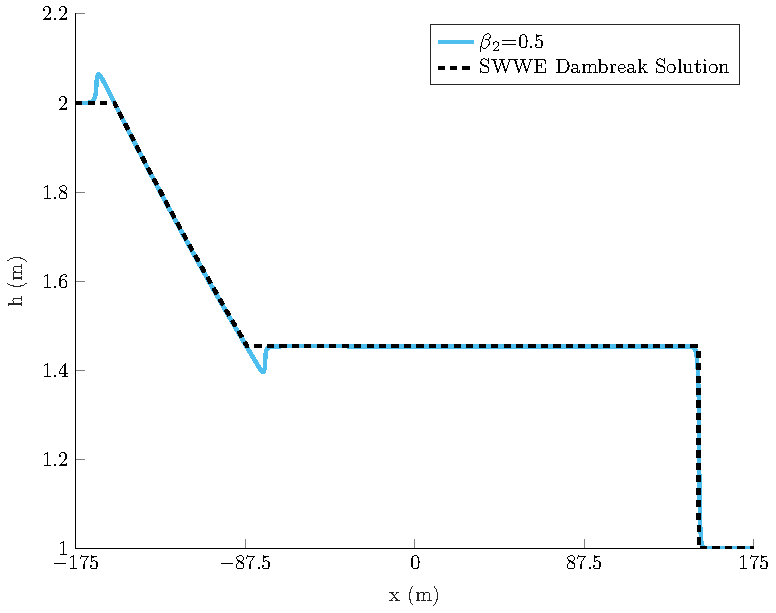
\includegraphics[width=\textwidth]{./Figures/Simulations/Study/RegSWWE/Convergence/h.pdf}
		\caption{$h$}
		\label{Fig:rSWWE_EX_h}
	\end{subfigure}
	\begin{subfigure}{0.32\textwidth}
		\centering
		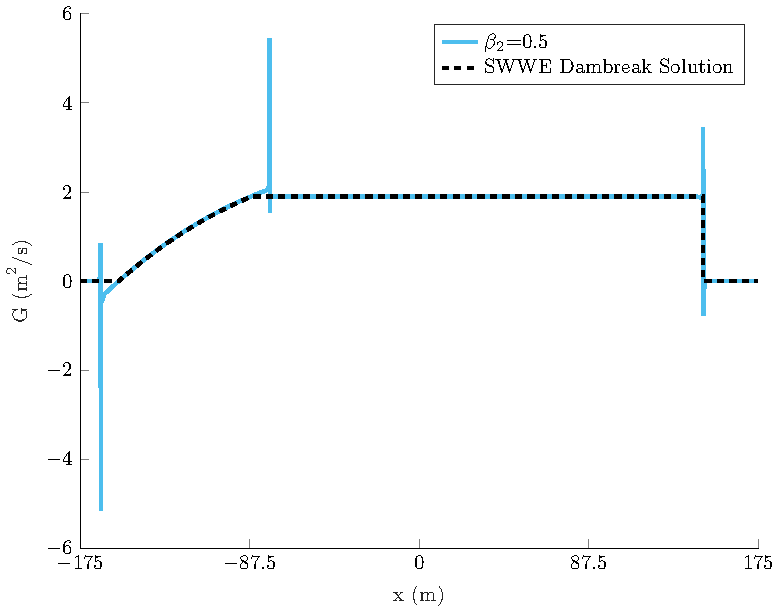
\includegraphics[width=\textwidth]{./Figures/Simulations/Study/RegSWWE/Convergence/G.pdf}
		\caption{$G$}
		\label{Fig:rSWWE_EX_G}
	\end{subfigure}
	\begin{subfigure}{0.32\textwidth}
		\centering
		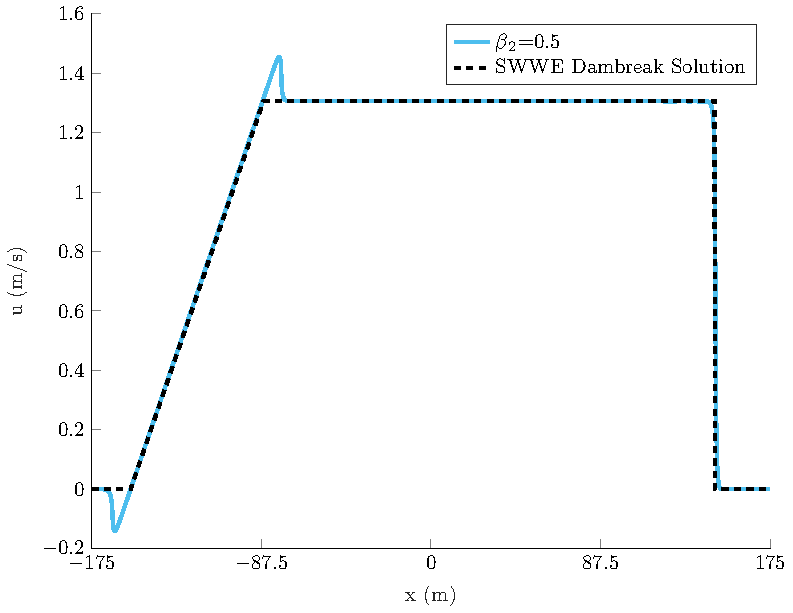
\includegraphics[width=\textwidth]{./Figures/Simulations/Study/RegSWWE/Convergence/u.pdf}
		\caption{$u$}
		\label{Fig:rSWWE_EX_u}
	\end{subfigure}
	\caption{Plot of example numerical solution for representative member of regularised SWWE family to smooth dam-break problem at $t=35s$.}
	\label{Fig:rSWWE_EX}
\end{figure}

In Figure \ref{Fig:rSWWE_EXS} the numerical solutions for $h$, $u$ and $G$ is shown for a number of members of the rSWWE family around important locations of the solution. These solutions demonstrate the convergence of this family of equations as $\beta_2 \rightarrow 0$, particularly for $G$ where the spikes are significantly damped. These results also verify that as shown by \cite{Dutykh-etal-2018-371}, that the shock speed of the rSWWE matches the shock speed of the SWWE.
%
\begin{figure}
	\centering
	\begin{subfigure}{0.32\textwidth}
		\centering
		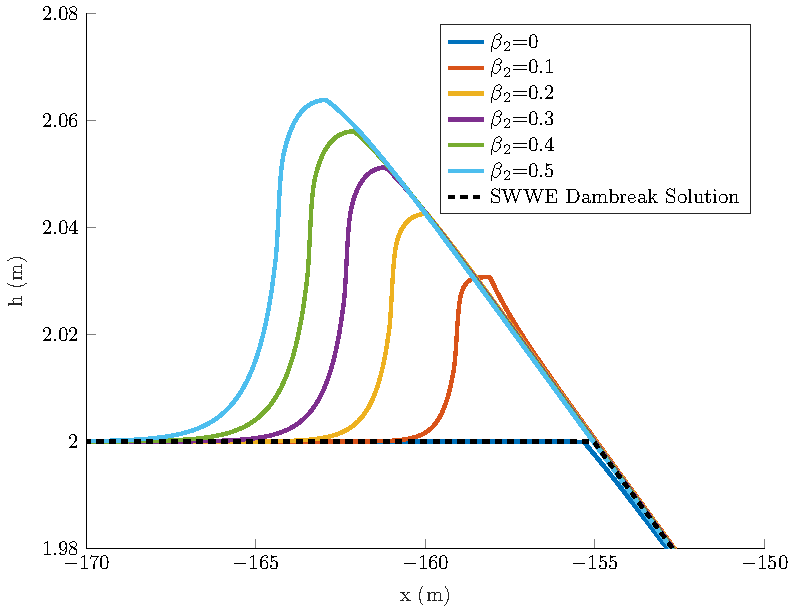
\includegraphics[width=\textwidth]{./Figures/Simulations/Study/RegSWWE/Convergence/hRFtop.pdf}
		\caption{$h$ top of rarefaction fan}
	\end{subfigure}
	\begin{subfigure}{0.32\textwidth}
		\centering
		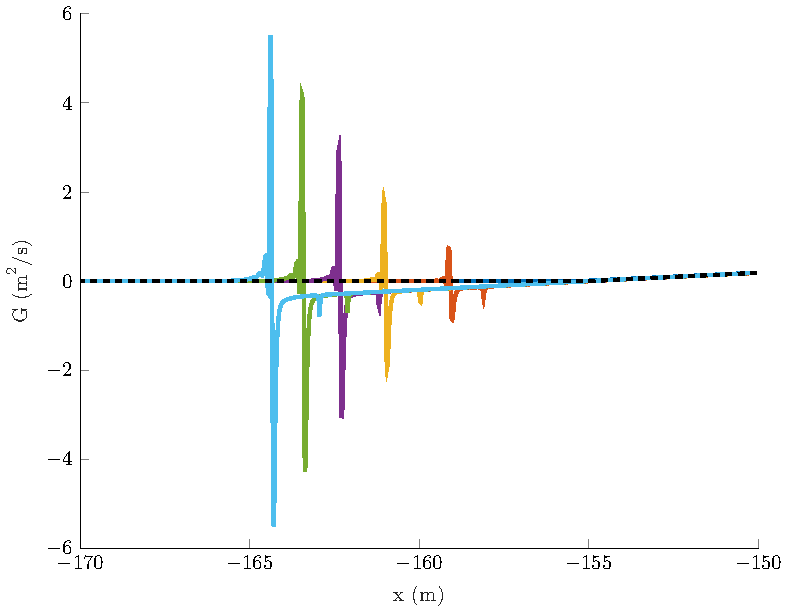
\includegraphics[width=\textwidth]{./Figures/Simulations/Study/RegSWWE/Convergence/GRFtop.pdf}
		\caption{$G$ top of rarefaction fan}
	\end{subfigure}
	\begin{subfigure}{0.32\textwidth}
		\centering
		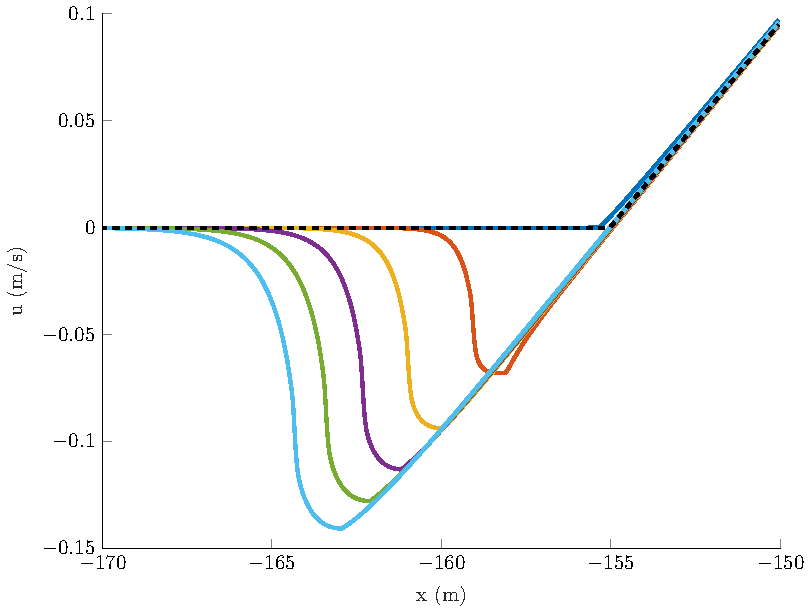
\includegraphics[width=\textwidth]{./Figures/Simulations/Study/RegSWWE/Convergence/uRFtop.pdf}
		\caption{$u$ top of rarefaction fan}
	\end{subfigure}
	\begin{subfigure}{0.32\textwidth}
		\centering
		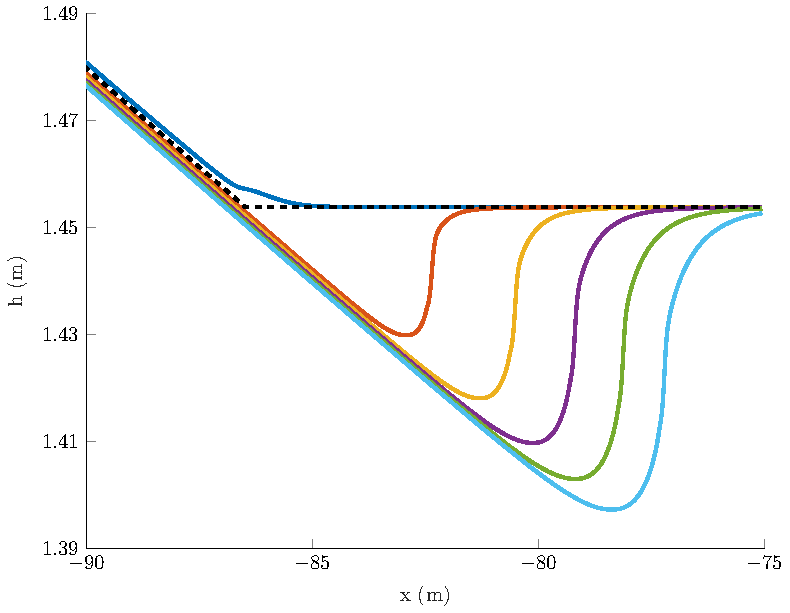
\includegraphics[width=\textwidth]{./Figures/Simulations/Study/RegSWWE/Convergence/hRFBot.pdf}
		\caption{$h$ bottom of rarefaction fan}
	\end{subfigure}
	\begin{subfigure}{0.32\textwidth}
		\centering
		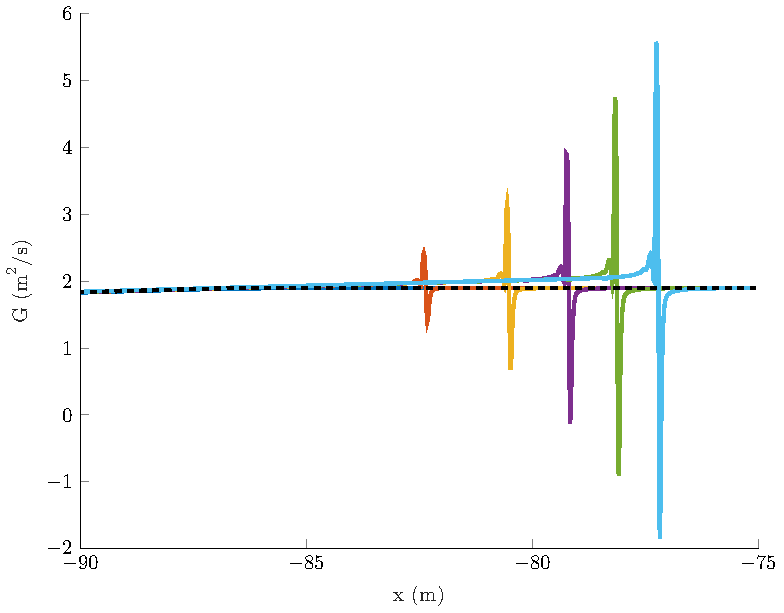
\includegraphics[width=\textwidth]{./Figures/Simulations/Study/RegSWWE/Convergence/GRFBot.pdf}
		\caption{$G$ bottom of rarefaction fan}
	\end{subfigure}
	\begin{subfigure}{0.32\textwidth}
		\centering
		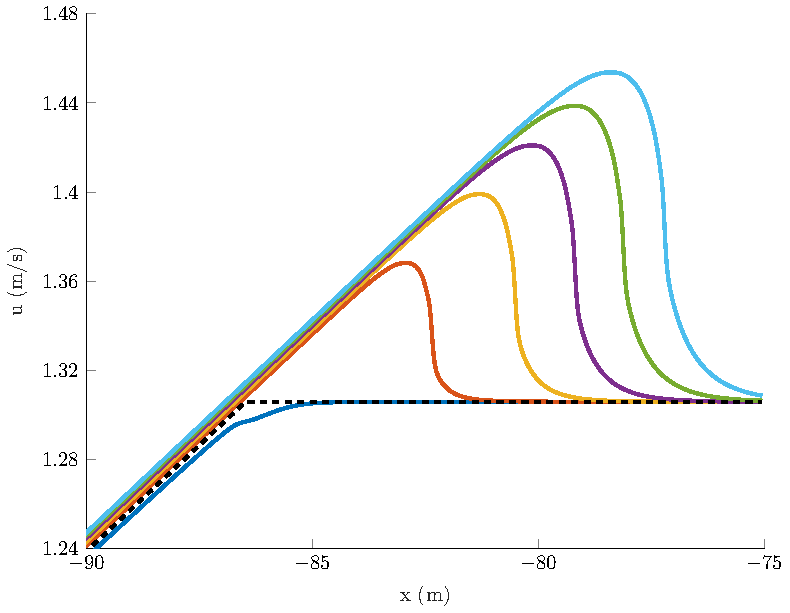
\includegraphics[width=\textwidth]{./Figures/Simulations/Study/RegSWWE/Convergence/uRFBot.pdf}
		\caption{$u$ bottom  of rarefaction fan}
	\end{subfigure}
	\begin{subfigure}{0.32\textwidth}
		\centering
		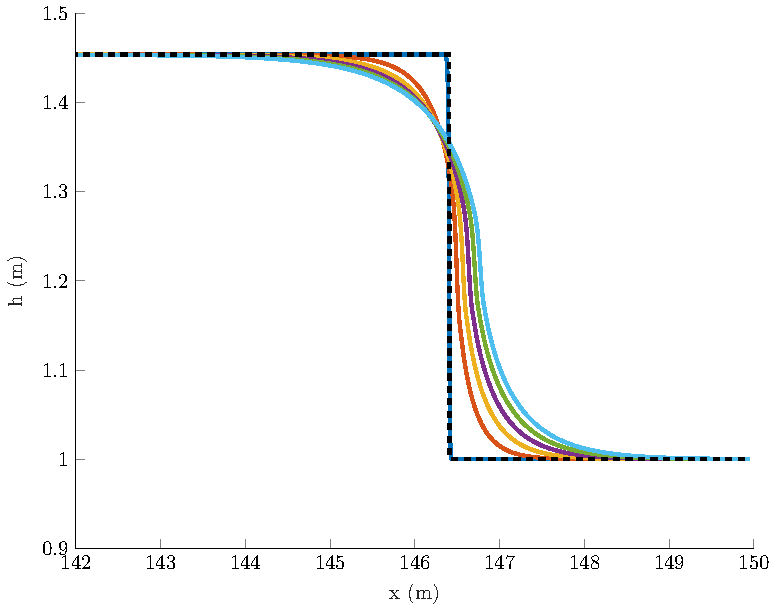
\includegraphics[width=\textwidth]{./Figures/Simulations/Study/RegSWWE/Convergence/hFront.pdf}
		\caption{$h$ shock front}
	\end{subfigure}
	\begin{subfigure}{0.32\textwidth}
		\centering
		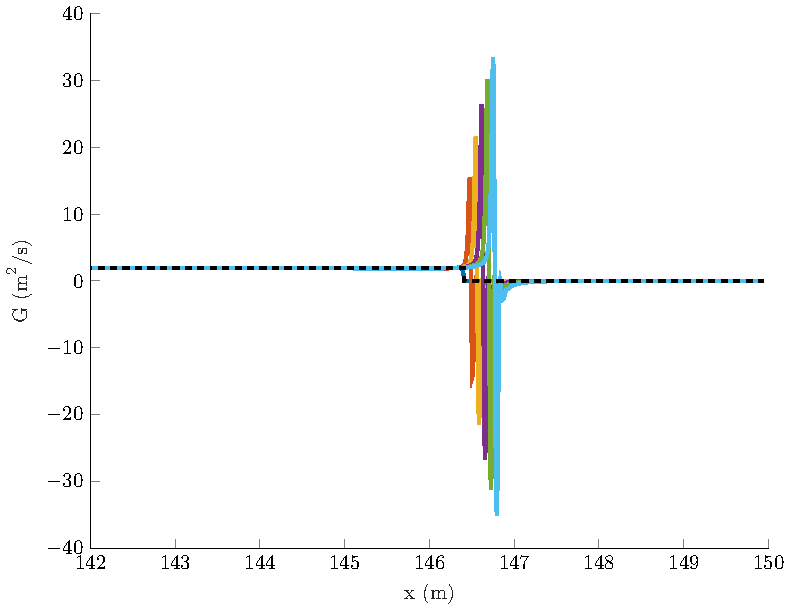
\includegraphics[width=\textwidth]{./Figures/Simulations/Study/RegSWWE/Convergence/GFront.pdf}
		\caption{$G$ shock front}
	\end{subfigure}
	\begin{subfigure}{0.32\textwidth}
		\centering
		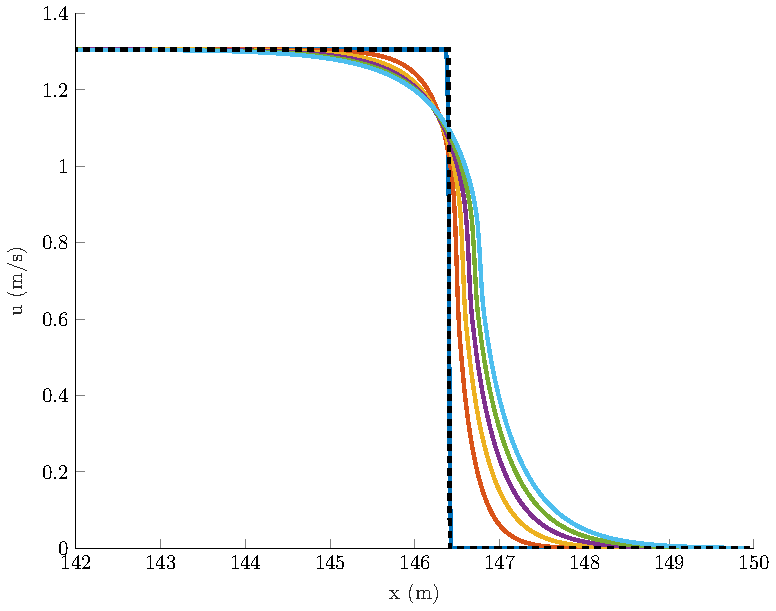
\includegraphics[width=\textwidth]{./Figures/Simulations/Study/RegSWWE/Convergence/uFront.pdf}
		\caption{$u$ shock front}
	\end{subfigure}
	\caption{Plot of multiple smooth dam-break numerical solutions at $t=35s$ with $\beta_2 = 0$ ({\color{mycolor1} \solidrule}), $\beta_2 = 0.1$ ({\color{mycolor2} \solidrule}), $\beta_2 = 0.2$ ({\color{mycolor3} \solidrule}), $\beta_2 = 0.3$ ({\color{mycolor4} \solidrule}), $\beta_2 = 0.4$ ({\color{mycolor5} \solidrule}), $\beta_2 = 0.5$ ({\color{mycolor6} \solidrule}) and the analytic solution of the SWWE to the dam-break problem (\dashedrule{}).} 
	\label{Fig:rSWWE_EXS}
\end{figure}

Table \ref{tab:rSWWE_Con} contains the conservation error \eqref{eqn:Cons_Error} for all the quantities conserved by the equations when the solutions are sufficiently smooth. Both $h$ and $G$ are conserved with only round-off errors by the numerical method. The momentum $uh$ is well conserved, particularly for the SWWE when $\beta_2 = 0$, but this conservation degrades as $\beta_2$ increases. The energy $\mathcal{E}$ is not very well conserved in the numerical solutions, this is due to the dissipation of energy in the equations \cite{Pu-2018-1361}. In Figure \ref{Fig:rSWWE_EnergyTime}, it is demonstrated that the energy dissipation occurs at the same rate as for the SWWE analytic solutions as demonstrated by \citet{Pu-2018-1361}. 
%
\begin{table}
	\centering
	\begin{tabular}{ c | c | c | c | c }
		$\beta_2$ & $h$ & $G$ & $uh$ & $\mathcal{E}$  \\
		\hline
		\T $0$ &	$5.8 \times 10^{-13}$ & $6.3 \times 10^{-13}$  & $6.3 \times 10^{-9}$ &	 $3.7 \times 10^{-3}$ \\
		\T $0.1$ &	$6.4 \times 10^{-13}$ & $6.4 \times 10^{-13}$  & $9.8 \times 10^{-6}$ &	 $3.9 \times 10^{-3}$ \\
		\T $0.2$ &	$6.7 \times 10^{-13}$ & $6.4 \times 10^{-13}$  & $1.1\times 10^{-5}$ &	 $4.1 \times 10^{-3}$ \\
		\T $0.3$ &	$6.9 \times 10^{-13}$ & $6.4 \times 10^{-13}$  & $1.2\times 10^{-5}$ &	 $4.3 \times 10^{-3}$ \\
		\T $0.4$ &	$7.1 \times 10^{-13}$ & $6.6 \times 10^{-13}$  & $1.2\times 10^{-5}$ &	 $4.4 \times 10^{-3}$ \\
		\T $0.5$ &	$7.1 \times 10^{-13}$ & $6.5 \times 10^{-13}$  & $1.3\times 10^{-5}$ &	 $4.6 \times 10^{-3}$ \\
	\end{tabular}
	\caption{Conservation errors $C_1$ for Regularised SWWE for the solutions provided above with $\beta_1 = \beta_2 - \frac{2}{3}$.}
	\label{tab:rSWWE_Con}
\end{table}
%
\begin{figure}
	\centering
	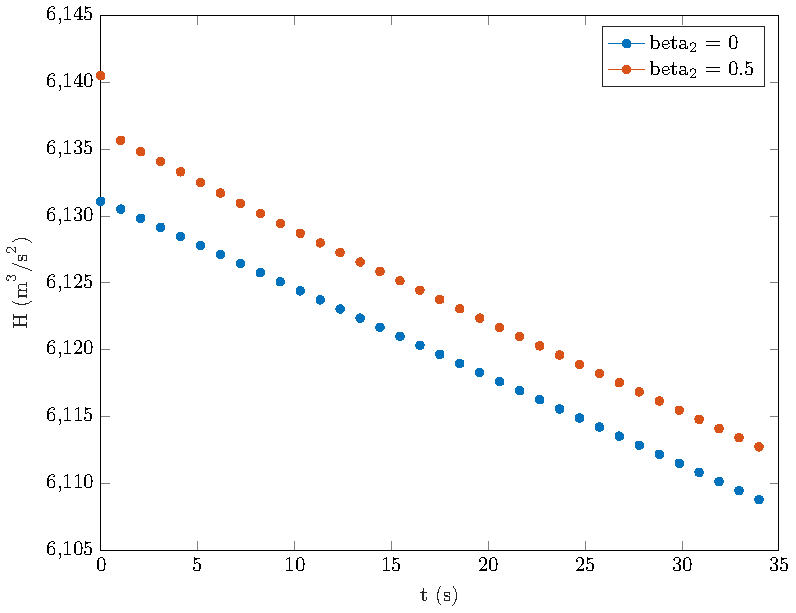
\includegraphics[width=0.6\textwidth]{./Figures/Simulations/Study/RegSWWE/Energy/EnergyOverTime.pdf}
	\caption{Total energy over time for the numerical solutions to the the rSWWE family with $\beta_2 = 0$ ({\color{mycolor1} \circlet{}}), $\beta_2 = 0.1$ ({\color{mycolor2} \squaret{}}), $\beta_2 = 0.2$ ({\color{mycolor3} \trianglet{}}), $\beta_2 = 0.3$ ({\color{mycolor4} \crosst{}}), $\beta_2 = 0.4$ ({\color{mycolor5} \circlet{}}), $\beta_2 = 0.5$ ({\color{mycolor6} \squaret{}}) and the analytic solution of the SWWE to the dam-break problem (\dashedrule{}).}
	\label{Fig:rSWWE_EnergyTime}
\end{figure}

These numerical results demonstrate that as $\beta_2 \rightarrow 0$ the numerical solutions nicely converge to the solution of the SWWE, and that the numerical method is capable of resolving solutions in the presence of the weak singularity, as desired.
%
\begin{itemize}
	\item we do get nice well behaved transitions between behaviours when varying $\beta$ values
	we get nice convergence.
	\item Although solutions look nice in h, in G there can be quite large values in the smoothed regions. However, u still looks quite nice. 
\end{itemize}
%
\subsection{The iSGN family ($\beta_2 = \beta_1$)}
The iSGN family of equations were derived by \citet{Clamond-et.al-2017-245} for the purpose of improving the dispersion relationship of the SGN equations without resorting to allowing higher powers of $\sigma$ in the approximation of the momentum equation. A particularly, important member of this family of equations corresponds to $\beta_1 = {2}/{15}$, which allows for the dispersion relationship of the iSGN to approximate the linear dispersion relationship of water waves up to order $O(k^6)$ for small $k$ \cite{Clamond-et.al-2017-245}. This is a significant improvement, and comes with only a relatively minor increase in complexity in the equations. The utility of this dispersion improvement was shown by \citet{Clamond-et.al-2017-245}. Therefore, how well the numerical method solves the iSGN and also what effect the free parameter has on the dispersive wave train, is of particular interest.  

Example numerical solutions for $h$, $G$ and $u$ with $\beta_1 = 0,\;1/15$ and $2/15 $ are plotted in Figure \ref{Fig:ImpDisp_EX}. The biggest difference between numerical solutions as $\beta$ varies is the clearing out of the middle of dispersive wave train as $\beta$ increases. This observation agrees well with the linear theory as can be see in Figure \ref{Fig:ImpDisp_LinWVSB} where the regions provided by the linear theory described in Table \ref{tab:rSWWE_LinearWaveSpeed}. Interestingly, even though the left and right sides of the dispersive wave train are fully separated when $\beta_1 \neq 0$  the growth in amplitude close to the wave speed bound as $k \rightarrow \infty$ observed for the SGN by \citet{Pitt-2018-61} can be seen for the members of the iSGN family. The wave train separation is not a feature of the linear theory of water waves \cite{Whitham-1967-399}, and so the better approximation provided by iSGN family, particularly for small $k$, is offset by this new behaviour in the limit as the wave number $k$ increases. However, for physical problems this is not an issue as physical effects not captured by the gSGN equations, will damp waves with large $k$ values.  
%
\begin{figure}
	\centering
	\begin{subfigure}{0.322\textwidth}
		\centering
		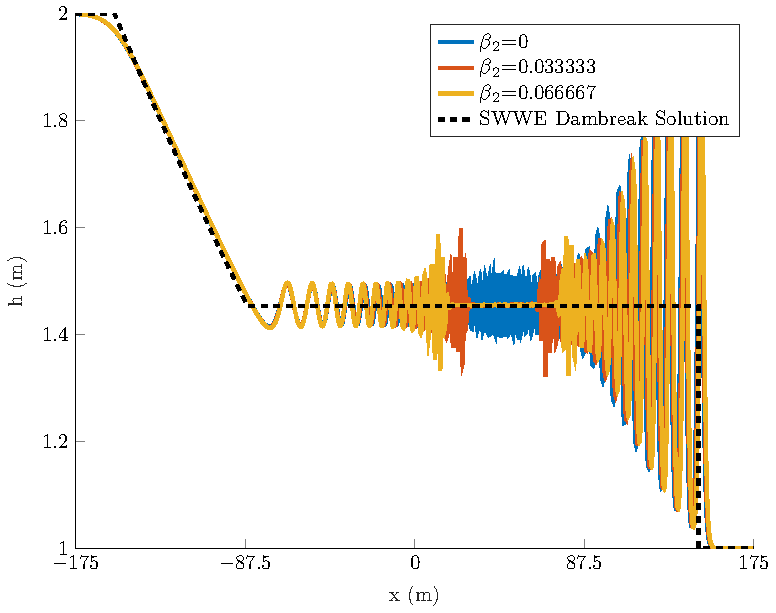
\includegraphics[width=\textwidth]{./Figures/Simulations/Study/ImpDisp/h.pdf}
		\caption{$h$}
	\end{subfigure}
	\begin{subfigure}{0.32\textwidth}
		\centering
		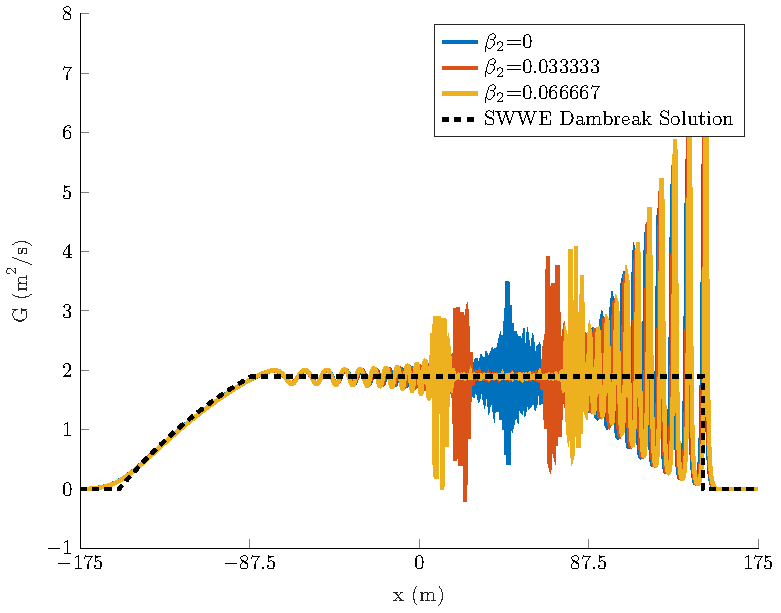
\includegraphics[width=\textwidth]{./Figures/Simulations/Study/ImpDisp/G.pdf}
		\caption{$G$}
	\end{subfigure}
	\begin{subfigure}{0.32\textwidth}
		\centering
		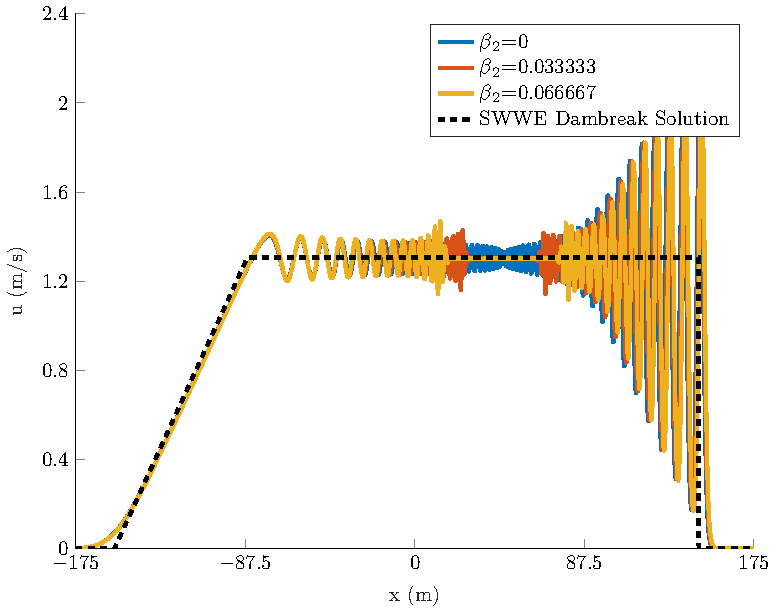
\includegraphics[width=\textwidth]{./Figures/Simulations/Study/ImpDisp/u.pdf}
		\caption{$u$}
	\end{subfigure}
	\caption{Plot of multiple smooth dam-break numerical solutions at $t=35s$ for members of the iSGN family of equations with $\beta_2 = 0$ ({\color{mycolor1} \solidrule}), $\beta_2 = 1/15$ ({\color{mycolor2} \solidrule}), $\beta_2 = 2/15$ ({\color{mycolor3} \solidrule}) and the analytic solution of the SWWE to the dam-break problem (\dashedrule{}).} 
	\label{Fig:ImpDisp_EX}
\end{figure}
%
%
%improve plots, want to plot more points, and use finer lines
\begin{figure}
	\centering
	\begin{subfigure}{0.49\textwidth}
		\centering
		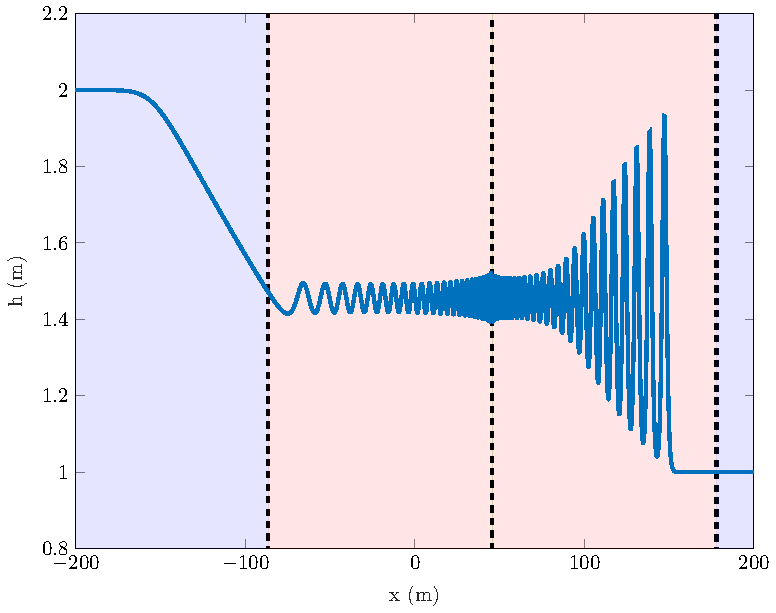
\includegraphics[width=\textwidth]{./Figures/Simulations/Study/ImpDisp/Regions/hRegionsSerre.pdf}
		\caption{$\beta_1 = \beta_2 = 0$}
	\end{subfigure}
	\begin{subfigure}{0.49\textwidth}
		\centering
		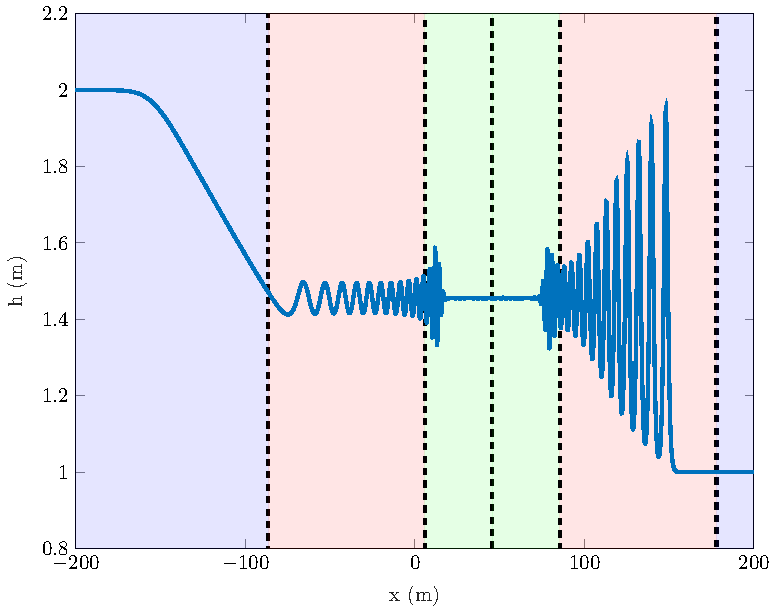
\includegraphics[width=\textwidth]{./Figures/Simulations/Study/ImpDisp/Regions/hRegionsImpDisp.pdf}
		\caption{$\beta_1 = \beta_2 = \frac{2}{15}$}
	\end{subfigure}
	\caption{Regions of wave speeds for the numerical solution to the smooth dam-break at $t=35s$ for significant members of the iSGN family.}
	\label{Fig:ImpDisp_LinWVSB}
\end{figure}
%
\begin{table}
	\centering
	\begin{tabular}{l | l | c}
		\T Colour region (left to right) & Description & Condition \\
		\hline
		\T first blue & beyond left wave speed bound &$\dfrac{x}{t} \le u_{2} - \sqrt{g h_{2}} $ \\
		\T first red & left dispersive wave train  & $  u_{2} - \sqrt{g h_{2}} \le \dfrac{x}{t} \le u_{2} - \sqrt{gh_{2}} \sqrt{\dfrac{\beta_2}{\frac{2}{3} + \beta_1}}$ \\
		\T first green & left flat region & $u_{2} - \sqrt{gh_{2}} \sqrt{\dfrac{\beta_2}{\frac{2}{3} + \beta_1}} \le \dfrac{x}{t} \le u_{2}$ \\
		\T second green & right flat region & $u_{2} \le \dfrac{x}{t}\le u_{2} + \sqrt{gh_{2}} \sqrt{\dfrac{\beta_2}{\frac{2}{3} + \beta_1}}$ \\
		\T second red & right dispersive wave train & $  u_{2} + \sqrt{gh_{2}} \sqrt{\dfrac{\beta_2}{\frac{2}{3} + \beta_1}} \le \dfrac{x}{t} \le  u_{2} + \sqrt{g h_{2}} $ \\
		\T second blue & beyond right wave speed bound & $u_{2} +  \sqrt{g h_{2}} \le \dfrac{x}{t} $ 	
	\end{tabular}
	\caption{Regions given by the linear wavespeed bounds for the constant state solution given by the SWWE \eqref{eq:SWWEMiddleState}.  	\label{tab:rSWWE_LinearWaveSpeed}  }
\end{table}

The most interesting regions when comparing numerical solutions of the iSGN equations are the middle and front of the dispersive wave train which have been plotted in Figure \ref{Fig:ImpDisp_EXZoom}. These results better demonstrate the growth in the amplitude around the 'contact discontinuity' \cite{Pitt-2018-61} with the plot of $G$ showing that when $\beta_1 \neq 0$, the limits of the dispersive wave train are even harder to resolve than for the SGN equations. Additionally, these figures show that as $\beta_1$ increases, so to does the speed and amplitude of the front of the dispersive wave train.
%
\begin{figure}
	\centering
	\begin{subfigure}{0.32\textwidth}
		\centering
		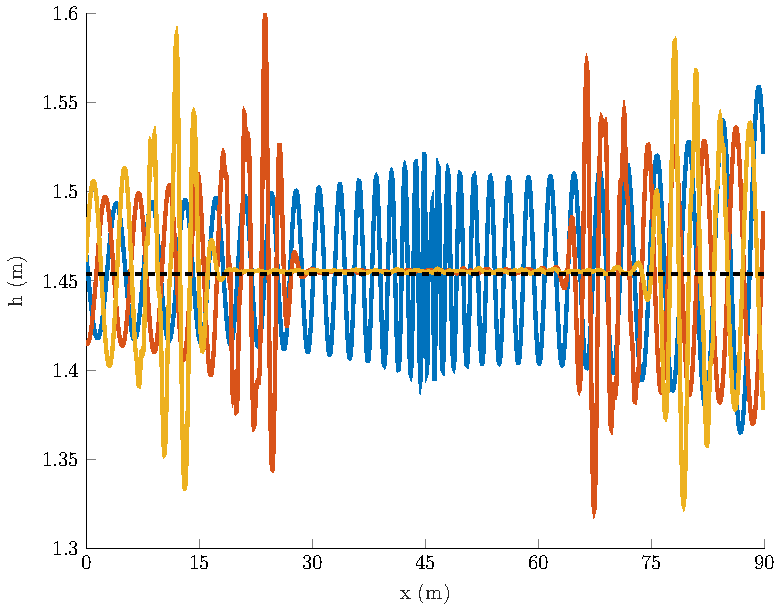
\includegraphics[width=\textwidth]{./Figures/Simulations/Study/ImpDisp/hMiddle.pdf}
		\caption{$h$ in middle of dispersive wave train}
	\end{subfigure}
	\begin{subfigure}{0.32\textwidth}
		\centering
		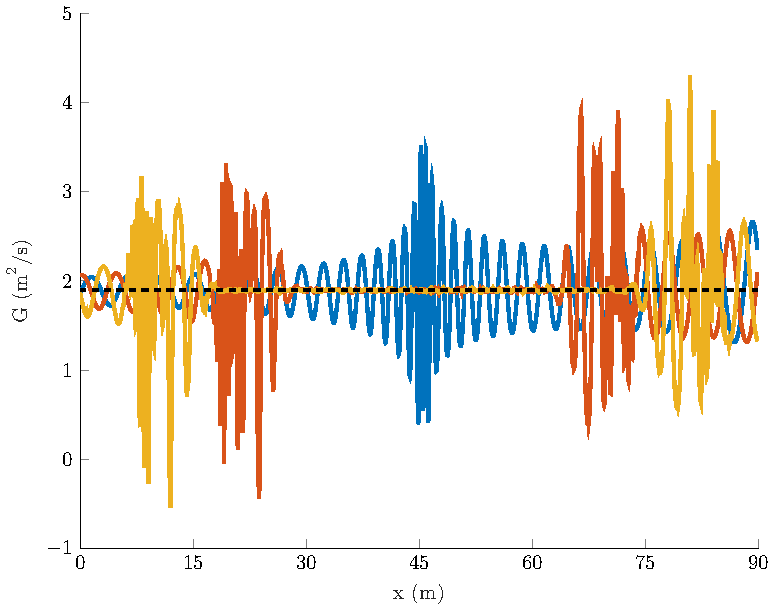
\includegraphics[width=\textwidth]{./Figures/Simulations/Study/ImpDisp/GMiddle.pdf}
		\caption{$G$ in middle of dispersive wave train}
	\end{subfigure}
	\begin{subfigure}{0.32\textwidth}
		\centering
		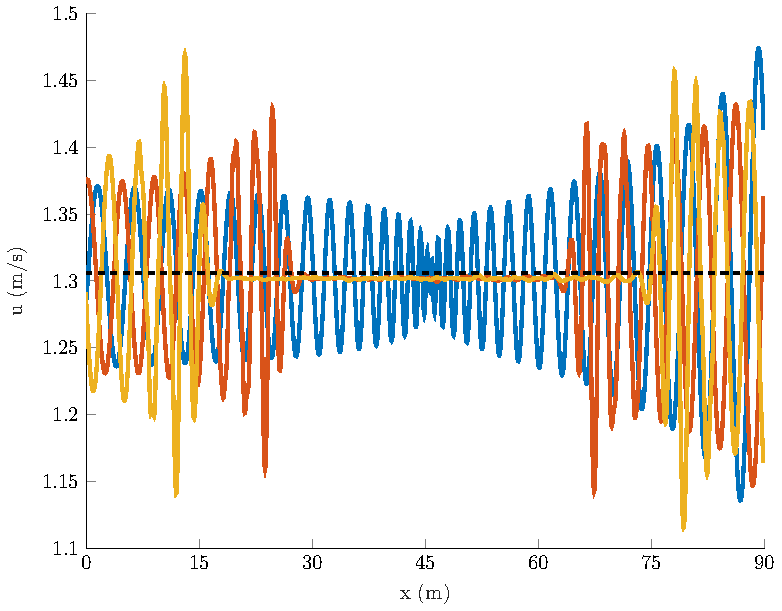
\includegraphics[width=\textwidth]{./Figures/Simulations/Study/ImpDisp/uMiddle.pdf}
		\caption{$u$ in middle of dispersive wave train}
	\end{subfigure}
	\begin{subfigure}{0.32\textwidth}
		\centering
		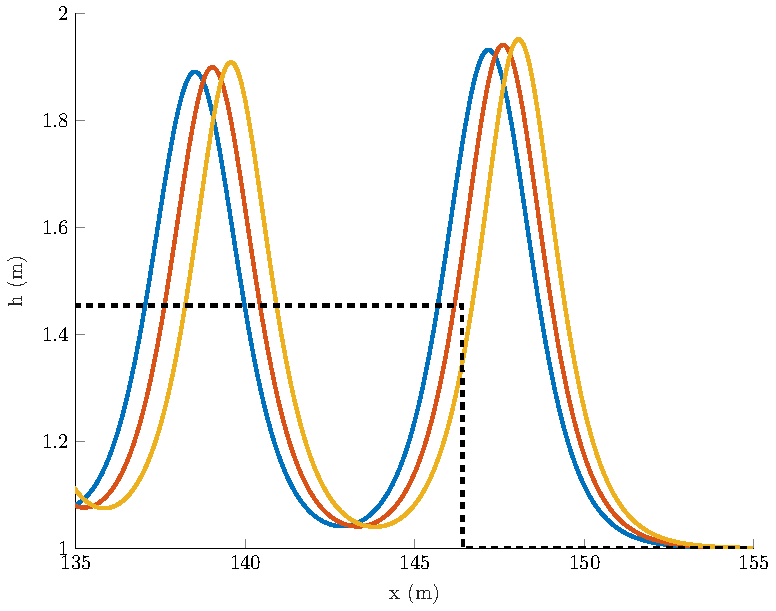
\includegraphics[width=\textwidth]{./Figures/Simulations/Study/ImpDisp/hFront.pdf}
		\caption{$h$ at front of dispersive wave train}
	\end{subfigure}
	\begin{subfigure}{0.32\textwidth}
		\centering
		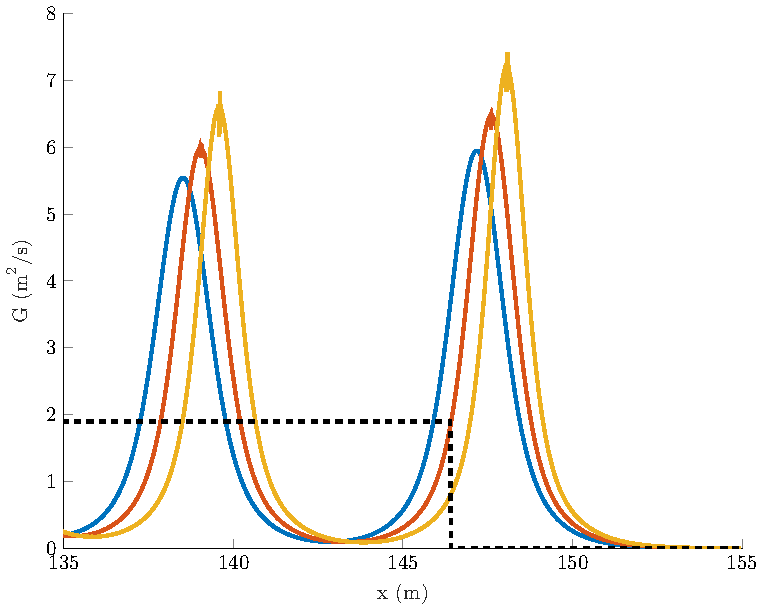
\includegraphics[width=\textwidth]{./Figures/Simulations/Study/ImpDisp/GFront.pdf}
		\caption{$G$ at front of dispersive wave train}
	\end{subfigure}
	\begin{subfigure}{0.32\textwidth}
		\centering
		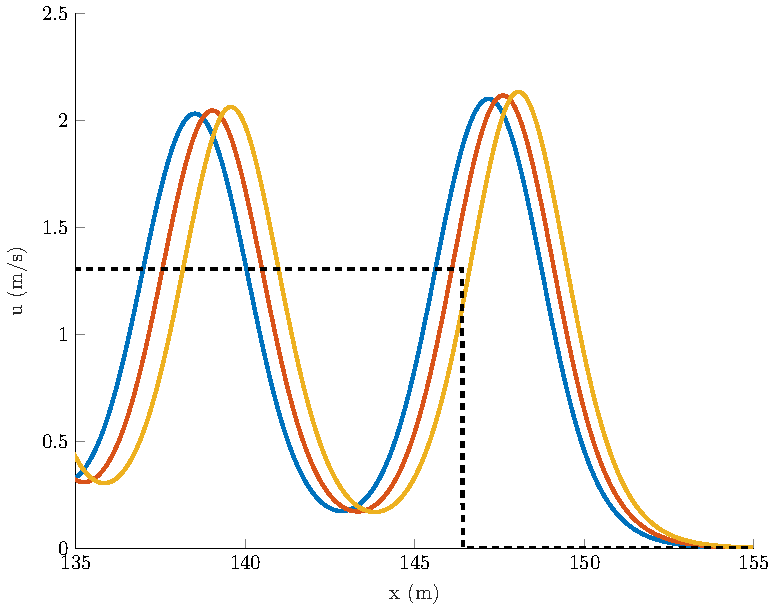
\includegraphics[width=\textwidth]{./Figures/Simulations/Study/ImpDisp/uFront.pdf}
		\caption{$u$ at front  of dispersive wave train}
	\end{subfigure}
	\caption{Plot of multiple smooth dam-break numerical solutions at $t=35s$ with $\beta_2 = 0$ ({\color{mycolor1} \solidrule}), $\beta_2 = 1/15$ ({\color{mycolor2} \solidrule}), $\beta_2 = 2/15$ ({\color{mycolor3} \solidrule}) and the analytic solution of the SWWE to the dam-break problem (\dashedrule{}).}
	\label{Fig:ImpDisp_EXZoom}
\end{figure}


Although the solutions of the iSGN equations appear to be more difficult to solve numerically, the conservation results in Table \ref{Tab:ImpDisp_Cons} remain quite good, even for the momentum $uh$. The conservation of energy $\mathcal{E}$ suffers due to the large gradients and low resolution of the solution around the dispersive wave limits. Unlike the rSWWE family, the conservation error in energy will decrease, as $\Delta x$ decreases and the numerical solutions better resolve these difficult locations.   
\begin{table}
	\centering
	\begin{tabular}{ c | c | c | c | c }
		$\beta_1$ & $h$ & $G$ & $uh$ & $\mathcal{E}$  \\
		\hline
		\T $0$ &	$8.0 \times 10^{-13}$ & $6.3 \times 10^{-13}$  & $3.3 \times 10^{-7}$ &	 $3.8 \times 10^{-6}$ \\
		\T${1}/{15}$ & $8.2 \times 10^{-13}$ &	$6.3 \times 10^{-13}$ & $5.8 \times 10^{-7}$	 &	$1.1 \times 10^{-5}$ \\
		\T${2}/{15}$ & $8.4 \times 10^{-13}$ &	$6.3 \times 10^{-13}$ & $9.1 \times 10^{-7}$	 &	$2.7 \times 10^{-4}$ \\
	\end{tabular}
	\caption{Conservation errors for Modified Dispersion Serre Equations for the solutions provided above with $\beta_2 = \beta_1 $.}
	\label{Tab:ImpDisp_Cons}
\end{table}
%

\begin{itemize}
	\item we do get nice well behaved transitions between behaviours when varying $\beta$
	\item Dispersive wave train location well approximated by using the linear wave speeds. Although the bump around these bounds suggests non-linear effects are important as well, particularly close to transitions across the wavespeed boundaries. 
	\item Improved dispersion may better approximate the dispsersion relation when $k\ll 1$, but at the cost of the middle of the dispersive wave train
	\item We get the bump behaviour observed in the db paper, but now dispersive wave trains are separate.
	\item Conservation is pretty similar, except for energy where it gets worse - this suggests that we will need finer grids to get good solutions particularly when gradients are large.
\end{itemize}

\subsection{SGN To SWWE Family $\beta_2 = 0$ and $-\frac{2}{3} \le \beta_1 \le 0$}
The family of equations that lie between the SGN equations and the SWWE, called the SGN to SWWE Family here, are important for understanding the effect of this dispersive term on the numerical solutions. Most notably many numerical methods that model dispersive waves rely on switching between the dispersive equations such as the SGN and the SWWE by turning on and off the dispersive term associated with $\beta_1$ \cite{Filippini-etal-2016-381,doCarmo-etal-2019-125}. Hitherto such switching has occurred heuristically, and was shown to provide good results for experimental results. The power of the gSGN family of equations and the associated numerical method is that some insight can be gained into the effect on numerical solutions, as dispersion is switched on and off. 

Investigating a wide array of $\beta_1$ values it was found that the most significant change occurred very close to the SWWE value of $\beta_1 = -2/3$. Therefore, the numerical solutions provided in the following figures are for $\beta_1$ values very close to the SWWE value, such as in the plots of $h$, $G$ and $u$ for numerical solutions in Figure \ref{Fig:SGN2SW_EX}. These figures show the effect of decreasing $\beta_1$ towards its SWWE value, which primarily affects the middle of the dispersive wave train dampening oscillations there. Eventually as $\beta_1$ is lowered further, the dispersive train is all but non-existent, although dispersive waves are observed around the shock and rarefaction fan. 
%
\begin{figure}
	\centering
	\begin{subfigure}{0.32\textwidth}
		\centering
		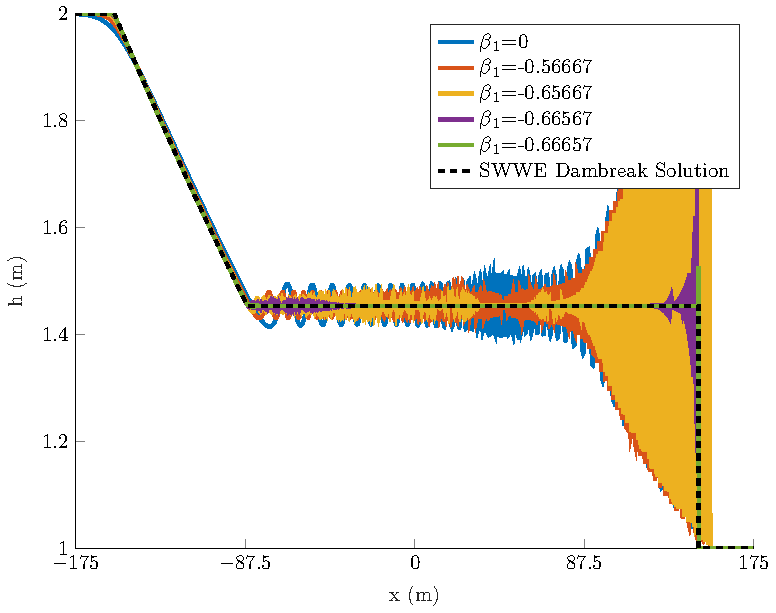
\includegraphics[width=\textwidth]{./Figures/Simulations/Study/Serre2SWWECloser/h.pdf}
		\caption{$h$}
	\end{subfigure}
	\begin{subfigure}{0.32\textwidth}
		\centering
		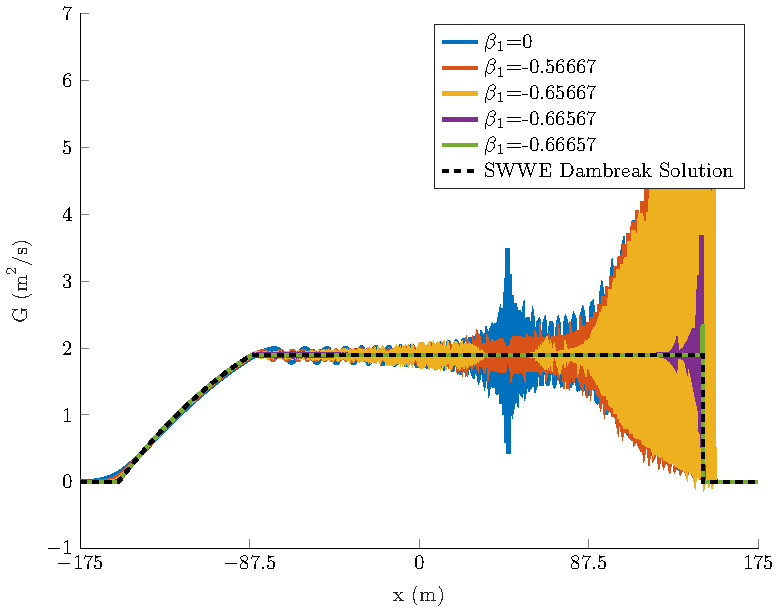
\includegraphics[width=\textwidth]{./Figures/Simulations/Study/Serre2SWWECloser/G.pdf}
		\caption{$G$}
	\end{subfigure}
	\begin{subfigure}{0.32\textwidth}
		\centering
		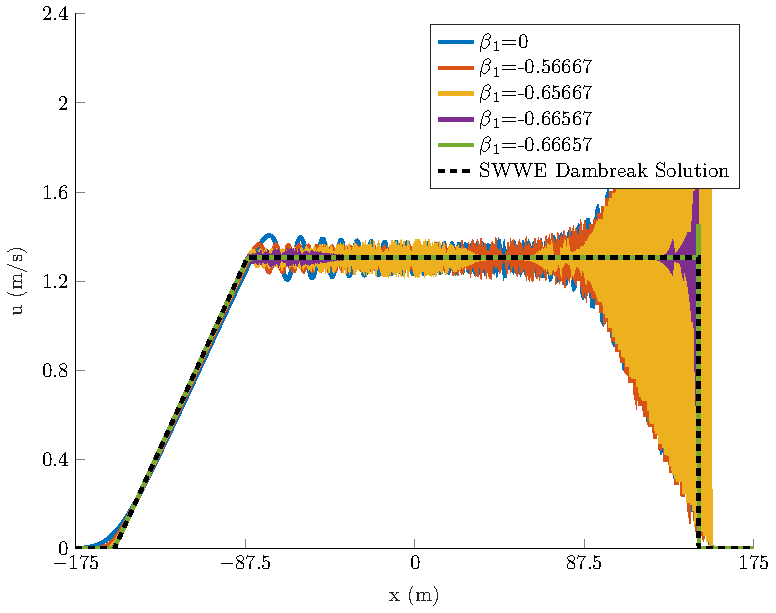
\includegraphics[width=\textwidth]{./Figures/Simulations/Study/Serre2SWWECloser/u.pdf}
		\caption{$u$}
	\end{subfigure}
	\caption{Plot of multiple smooth dam-break numerical solutions at $t=35s$ for members of the SGN to SWWE family with $\beta_1 = 0$ ({\color{mycolor1} \solidrule}), $\beta_1 = -2/3 + 10^{-1}$ ({\color{mycolor2} \solidrule}), $\beta_1 = -2/3 + 10^{-2}$  ({\color{mycolor3} \solidrule}), $\beta_1 = -2/3 + 10^{-3}$  ({\color{mycolor4} \solidrule}), $\beta_1 = -2/3 + 10^{-4}$ ({\color{mycolor5} \solidrule}) and the analytic solution of the SWWE to the dam-break problem (\dashedrule{}).}
	\label{Fig:SGN2SW_EX}
\end{figure}

The finer structure of the solutions can be seen in Figure \ref{Fig:SGN2SW_EXXoom} around the middle and front of the dispersive wave train. The frequency and thus the wave-number of the dispersive wave train increases dramatically as $\beta_1$ approaches $-2/3$, this is because the dispersive term is very small for all but the steepest gradients, and thus the lower frequency waves are removed leaving only the high frequency ones. However, this only occurs very close to $\beta_1$'s critical value with extensive dispersive wave trains observed for most of the SGN To SWWE family. The removal of the dispersive wave train is not due to the emergence and growth of the non-dispersive region as in the iSGN family, as can be seen in Figure \ref{Fig:SGN2SW_Regions} which plots the regions of linear wavespeed described in Table \ref{tab:rSWWE_LinearWaveSpeed} over the numerical solution. 
%
\begin{figure}
	\centering
	\begin{subfigure}{0.32\textwidth}
		\centering
		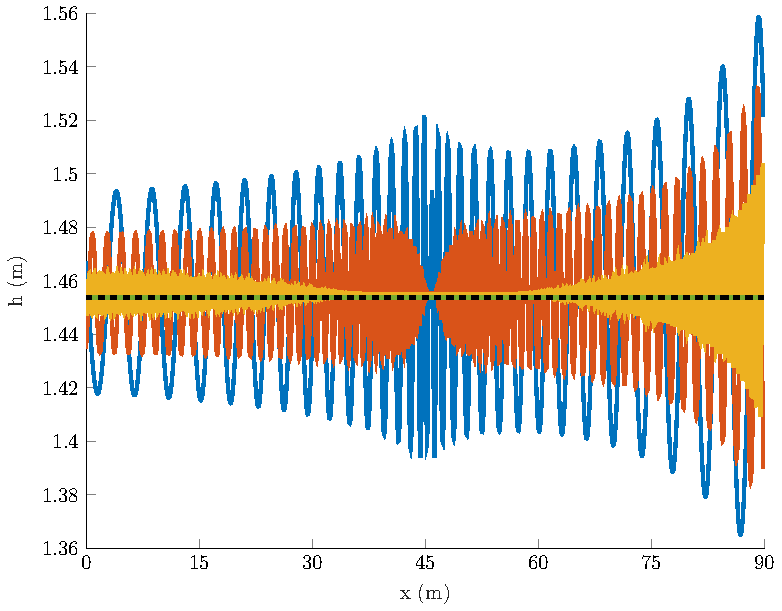
\includegraphics[width=\textwidth]{./Figures/Simulations/Study/Serre2SWWECloser/hMid.pdf}
		\caption{$h$ middle of dispersive wave train}
	\end{subfigure}
	\begin{subfigure}{0.32\textwidth}
		\centering
		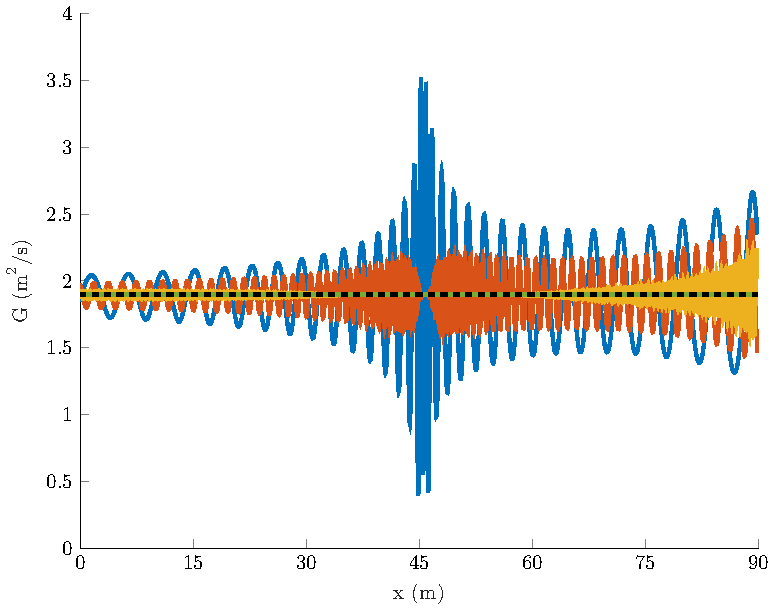
\includegraphics[width=\textwidth]{./Figures/Simulations/Study/Serre2SWWECloser/GMid.pdf}
		\caption{$G$ middle of dispersive wave train}
	\end{subfigure}
	\begin{subfigure}{0.32\textwidth}
		\centering
		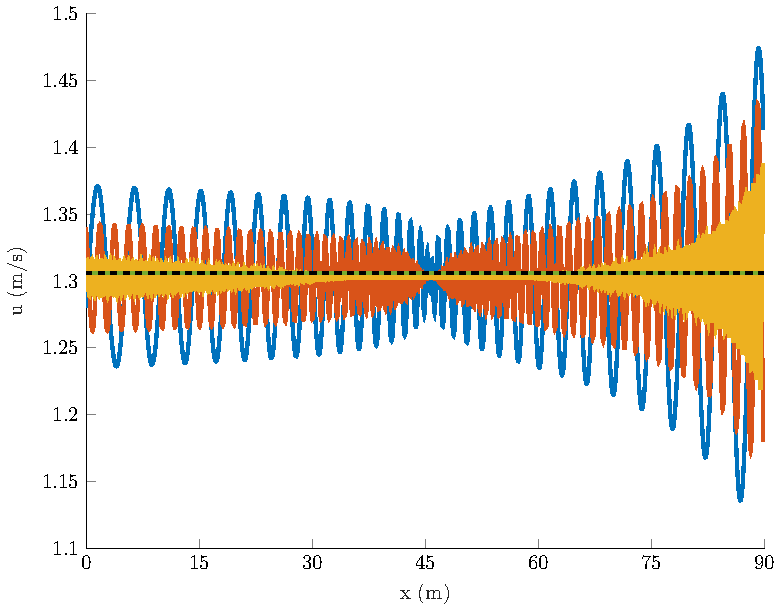
\includegraphics[width=\textwidth]{./Figures/Simulations/Study/Serre2SWWECloser/uMiddle.pdf}
		\caption{$u$ middle of dispersive wave train}
	\end{subfigure}
	\begin{subfigure}{0.32\textwidth}
		\centering
		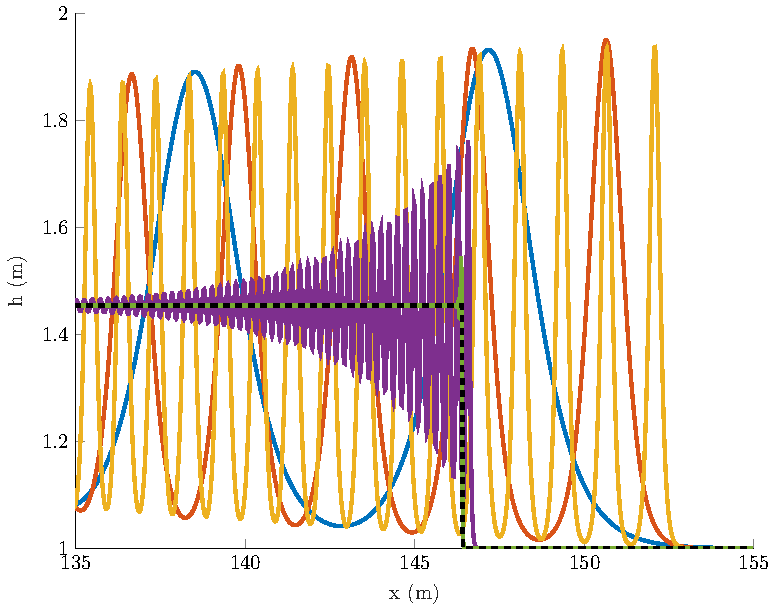
\includegraphics[width=\textwidth]{./Figures/Simulations/Study/Serre2SWWECloser/hFront.pdf}
		\caption{$h$ front of dispersive wave train}
	\end{subfigure}
	\begin{subfigure}{0.32\textwidth}
		\centering
		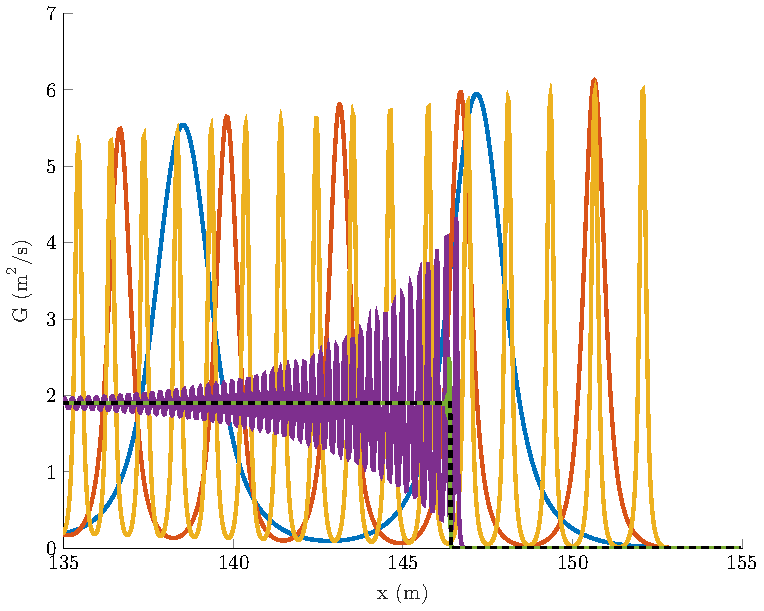
\includegraphics[width=\textwidth]{./Figures/Simulations/Study/Serre2SWWECloser/GFront.pdf}
		\caption{$G$ front of dispersive wave train}
	\end{subfigure}
	\begin{subfigure}{0.32\textwidth}
		\centering
		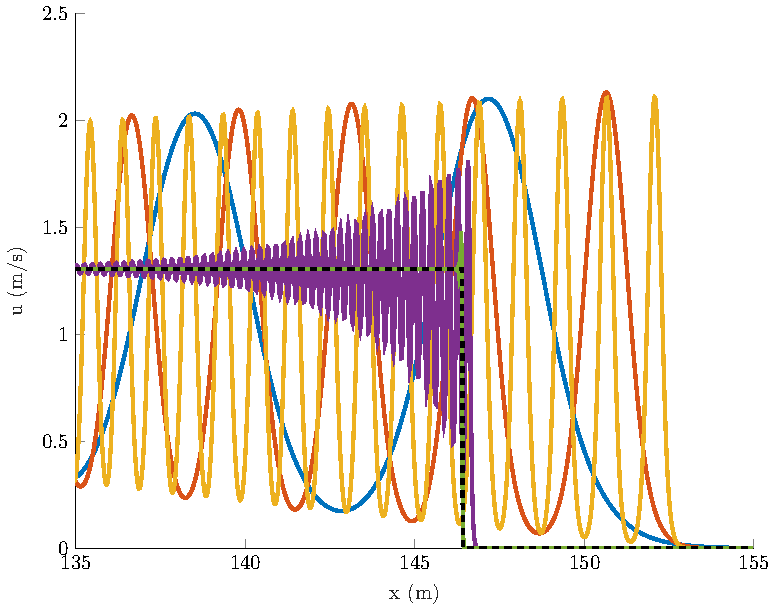
\includegraphics[width=\textwidth]{./Figures/Simulations/Study/Serre2SWWECloser/uFront.pdf}
		\caption{$u$ front of dispersive wave train}
	\end{subfigure}
	\caption{Plot of multiple smooth dam-break numerical solutions at $t=35s$ for members of the SGN to SWWE family with $\beta_1 = 0$ ({\color{mycolor1} \solidrule}), $\beta_1 = -2/3 + 10^{-1}$ ({\color{mycolor2} \solidrule}), $\beta_1 = -2/3 + 10^{-2}$  ({\color{mycolor3} \solidrule}), $\beta_1 = -2/3 + 10^{-3}$  ({\color{mycolor4} \solidrule}), $\beta_1 = -2/3 + 10^{-4}$ ({\color{mycolor5} \solidrule}) and the analytic solution of the SWWE to the dam-break problem (\dashedrule{}) around important locations.}
	\label{Fig:SGN2SW_EXXoom}
\end{figure}
%
\begin{figure}
	\centering
	\begin{subfigure}{0.49\textwidth}
		\centering
		\includegraphics[width=\textwidth]{./Figures/Simulations/Study/Serre2SWWECloser/Regions/hRegionsSerre.pdf}
		\caption{$\beta_1 = \beta_2 = 0$}
	\end{subfigure}
	\begin{subfigure}{0.49\textwidth}
		\centering
		\includegraphics[width=\textwidth]{./Figures/Simulations/Study/Serre2SWWECloser/Regions/hRegionsSerreSWWEClose.pdf}
		\caption{$\beta_1 = -\frac{2}{3} + 10^{-3}$ and  $\beta_2 = 0$}
	\end{subfigure}
	\caption{Regions of wave speeds for the smooth dambreak numerical solution at $t=35s$.}
	\label{Fig:SGN2SW_Regions}
\end{figure}

The conservation of all quantities of interest are summarised in Table \ref{Tab:SGN2SW_Cons}. As observed for all numerical solutions, $h$ and $G$ are conserved by the numerical method up to round-off error for all values of $\beta_1$. The momentum is well conserved for numerical solutions of both the SGN equations and the SWWE, but is poorest for intermediate values of $\beta_1$. The conservation of energy however gets worse, as $\beta_1$ approaches the critical value and the dissipation of energy very quickly becomes the same as for the SWWE, as seen in Figure \ref{Fig:SGN2SW__EnergyTime}. 
%
\begin{table}
	\centering
	\begin{tabular}{ c | c | c | c | c }
		$\beta_1$ & $h$ & $G$ & $uh$ & $\mathcal{H}$  \\
		\hline
		\T $0$ &	$8.0 \times 10^{-13}$ &	$6.3 \times 10^{-13}$ & $3.3 \times 10^{-7}$ & $3.8 \times 10^{-6}$ \\
		\T $-{2}/{3} + 10^{-1}$ &	$7.2 \times 10^{-13}$ &	$6.3 \times 10^{-13}$ & $3.0 \times 10^{-6}$ & $6.3 \times 10^{-6}$ \\
		\T $-{2}/{3} + 10^{-2}$ &	$6.6 \times 10^{-13}$ &	$6.2 \times 10^{-13}$ & $3.2 \times 10^{-5}$ & $3.7 \times 10^{-4}$ \\		
		\T $-{2}/{3} + 10^{-3}$ &	$6.0 \times 10^{-13}$ &	$6.3 \times 10^{-13}$ & $1.2 \times 10^{-5}$ & $3.7 \times 10^{-3}$ \\	
		\T $-{2}/{3} + 10^{-4}$ &	$5.9 \times 10^{-13}$ &	$6.2 \times 10^{-13}$ & $1.2 \times 10^{-6}$ & $3.7 \times 10^{-3}$ \\
		\T $-{2}/{3} $ &	$5.8 \times 10^{-13}$ & $6.3 \times 10^{-13}$  & $6.3 \times 10^{-9}$ &	 $3.7 \times 10^{-3}$ \\		
	\end{tabular}
	\caption{Conservation errors for Serre To SWWE Family of Equations for the solutions provided above with $\beta_2 = 0$ and $-\frac{2}{3}\le \beta_1 \le 0$.}
	\label{Tab:SGN2SW_Cons}
\end{table}
%
\begin{figure}
	\centering
	\includegraphics[width=0.6\textwidth]{./Figures/Simulations/Study/Serre2SWWECloser/Energy/EnergyOverTime.pdf}
	\caption{Total energy over time for the numerical solutions to the SGN to SWWE family with $\beta_1 = 0$ ({\color{mycolor1} \circlet{}}), $\beta_1 = -2/3 + 10^{-1}$ ({\color{mycolor2} \squaret{}}), $\beta_1 = -2/3 + 10^{-2}$ ({\color{mycolor3} \trianglet{}}), $\beta_1 = -2/3 + 10^{-3}$ ({\color{mycolor4} \crosst{}}), $\beta_1 = -2/3 + 10^{-4}$ ({\color{mycolor5} \circlet{}}) and the analytic solution of the SWWE to the dam-break problem (\solidrule{}).}
	\label{Fig:SGN2SW__EnergyTime}
\end{figure}

Points:
\begin{itemize}
	\item we do get convergence, but most of the convergent behaviour occurs very close to the critical SWWE value. This is because gradients are large in the initial conditions
	\item Middle of dispersive wave train, and base and top of rarefaction fan most affected (closer to Serre)
	\item Still quite a large dispersive wave train even for $\beta_1$ values close to $-2/3$. (This appears to justify switching)
	\item the front of the shock became larger for some intermediate values.
	\item Trade-off between momentum convergence (since G = uh for SWWE) and energy convergence. Dispersive models conserve energy better due to smooth solutions, but conserve momentum worse because conserved quantity is not uh. 
\end{itemize}

\section{Conclusion}
A modified version of the SGN solver outlined by \citet{Zoppou-etal-2017} was used to solved the gSGN equations which make the constant in front of the dispersive term free and adds a surface tension-like regularisation term \cite{Clamond-et.al-2017-245,Clamond-Dutykh-2018-237}. The new gSGN solver was validated against analytic solutions of the SGN and SWWE equations and forced solutions. The analytic solutions demonstrate that the gSGN solver accurately reproduces important members of the gSGN family of equations whilst conserving the quantities of interest for sufficiently smooth solutions, and the forced solutions demonstrate that the method remains second-order for all values of the free parameters, $\beta_1$ and $\beta_2$. The gSGN method described above is the first well validated numerical method for the gSGN equations and the rSWWE and iSGN families of equations. The numerical method is then used to verify and expand numerical results in the literature for the smoothed dam-break problem \cite{Clamond-Dutykh-2018-237,Clamond-et.al-2017-245,Pu-2018-1361}. The first set of these experiments demonstrate the rSWWE family possesses regularised numerical solutions that converge nicely as the SWWE are approached. Additionally, the numerical results for energy dissipation agree with the analytic result of \citet{Pu-2018-1361}, where the weak singularities associated with this dissipation can be seen in plots of the conserved quantity $G$. The second group of experiments demonstrate the behaviour of the iSGN family of equations, which agrees very well with the linear theory. The results demonstrate that for steep gradient problems the iSGN family will require higher resolution grids or higher order methods to resolve the dispersive wave train around the high wave-number limits. Finally, the numerical solutions for the family of equations that lie between the SGN and SWWE equations, the SGN to SWWE family were studied. These results demonstrate that even for very small $\beta_1$ values steep gradients will develop extensive dispersive wave trains and when $\beta_1$ is close to the critical SWWE value, then the solutions of the SGN to SWWE family dissipate energy at the same rate as the SWWE for the numerical solutions. 

\section{References}
\bibliographystyle{unsrtnat}
\bibliography{Bibliography}


\end{document} 